\documentclass[11pt,letterpaper]{article}

\usepackage[T1]{fontenc}
\usepackage{lmodern}
\usepackage{microtype}
\usepackage[margin=1in]{geometry}      % one-inch margins, as the writing standard specifies
\linespread{1.0}
\setlength{\parskip}{0pt}          % conventional article: indent, no vertical gap
\setlength{\parindent}{1.5em}

\usepackage{amsmath,amssymb,amsthm}
\usepackage{graphicx}
\usepackage{xcolor}
\usepackage{tikz}
\usepackage{booktabs,tabularx,array,longtable}
\newcolumntype{L}[1]{>{\raggedright\arraybackslash}p{#1}}
\newcolumntype{Y}{>{\raggedright\arraybackslash}X}
\usepackage{listings}
\lstset{basicstyle=\ttfamily\footnotesize,breaklines=true,columns=fullflexible,frame=single,framesep=4pt,showstringspaces=false,captionpos=b}
\usepackage[round,authoryear]{natbib}
\usepackage[hidelinks]{hyperref}
\usepackage{cleveref}

\definecolor{grokgray}{RGB}{110,110,110}
\AddToHook{shipout/background}{%
  \ifnum\value{page}=1
    \put(30pt,-0.5\paperheight){\makebox(0,0){\rotatebox{90}{\footnotesize\sffamily\color{grokgray}%
      GrokRxiv:2026.10.productive-power\quad [\,econ.GN\,]\quad 22 Oct 2026}}}%
  \fi
}

\newtheorem{theorem}{Theorem}[section]
\newtheorem{proposition}[theorem]{Proposition}
\newtheorem{lemma}[theorem]{Lemma}
\newtheorem{corollary}[theorem]{Corollary}
\theoremstyle{definition}
\newtheorem{definition}[theorem]{Definition}
\newtheorem{assumption}[theorem]{Assumption}
\theoremstyle{remark}
\newtheorem{remark}[theorem]{Remark}

\crefname{assumption}{Assumption}{Assumptions}

% Pillar labels (sans-serif, series convention) and shared objects
\newcommand{\pF}{\mathsf{F}}
\newcommand{\pP}{\mathsf{P}}
\newcommand{\pJ}{\mathsf{J}}
\newcommand{\pI}{\mathsf{I}}
\newcommand{\pC}{\mathsf{C}}
\newcommand{\pW}{\mathsf{W}}
\newcommand{\Pill}{\mathcal{M}}
\newcommand{\Integ}{\mathcal{I}}
\newcommand{\QW}{Q^{\pW}}
\newcommand{\HW}{H_{\pW}}

\title{Productive Power and Social Reproduction\\[4pt]
  {\normalsize Part VI of \emph{The Six Pillars of the Beast System}}}
\author{Matthew Long\\
  \small The YonedaAI Collaboration, YonedaAI Research Collective\\
  \small Chicago, IL\\
  \small \texttt{matthew@yonedaai.com} \quad \url{https://yonedaai.com}}
\date{October 2026}

\begin{document}
\maketitle

\begin{abstract}
Every governance system consumes resources that someone must produce. This paper treats production, payment and social reproduction as the sixth pillar of a comparative framework in which six functions (resource allocation, rule-making, adjudication, legitimation, sanction and production) are present in every functioning polity. From a maintenance axiom we prove that a persistent collective must produce at a positive average rate and must reproduce its producers through care labor, and that rents, tribute, migration or automation relocate production rather than remove it. The same dependence gives producers a latent veto: when outside revenue falls short of the institutions' maintenance requirement, a collective withdrawal of labor, taxes or trade threatens their persistence. A bargaining model makes the channels exact. Producers' terms rise with their outside option and organized bargaining weight, fall linearly with the concentration of control over productive participation, and lose their withdrawal premium once rents cover the maintenance requirement. Restricting mobility pays only when the value of free exit exceeds the cost of enforcement, a condition that nests Domar's land-labor hypothesis and Brenner's emphasis on class organization. Every instrument that depresses producers' terms is held in another pillar, so the capture of production never originates inside it. A comparison of six regime types finds the function everywhere and its capture only under specific couplings. Read typologically, Revelation 13:16 and 17 depict the limiting case in which exchange is conditioned on allegiance. The parameters are not estimated here; nine hypotheses state what would falsify the model.
\end{abstract}

\section{Introduction}
\label{sec:intro}

This paper asks who produces the wealth that sustains everything. The question is older than political economy, but it is usually asked in one of two narrow forms. Economists ask how output is divided among wages, profits, rents and taxes. Political scientists ask when those who pay taxes obtain representation. Both forms take for granted something this paper makes explicit: that every governance system, whatever its ideology, runs on a flow of goods and services that its rulers do not themselves produce in sufficient quantity, and that the people who do produce it therefore hold a form of power that no ruler can abolish, only channel, divide or suppress.

The paper is Part VI of a seven-part series on the six functions that every governance system must perform. The series follows \citet{largo2026hbs}, who proposed a multiplex network model of five institutional functions under the name ``Hierarchy of the Beast System.'' The series splits Largo's rule function into rule-making and adjudication, giving six pillars: financial power $\pF$ (who controls the resources), political power $\pP$ (who makes the laws), judicial power $\pJ$ (who interprets the laws), ideological power $\pI$ (who shapes the beliefs), coercive power $\pC$ (who enforces the rules) and productive power $\pW$ (who produces the wealth that sustains everything). The thesis of the series is that the ideology changes and the institutional functions remain. ``Beast System'' names that universal six-function structure. It is never a label for a religion, a people, a profession, a regime or a person.

Two propositions organize the series and must be kept apart. Proposition A, proved in general in Part VII \citep{long2026formalized}, states that every functioning governance system contains all six functions together with dependency relations among them. Proposition B describes capture: the functions become concentrated or coordinated so that independent accountability fails. Proposition B is contingent and measurable, and Part VII proves that A does not imply B. Each pillar paper derives its own pillar from one axiom, shows the pillar's minimal form in stateless and consensus societies, compares how the function is distributed across six regime types, and states when coordination in the pillar becomes capture.

For production the derivation is short and the consequences are not. The maintenance axiom says that the group and its institutions consume resources that someone produces. From it we prove that a persistent collective must implement production at a positive average rate (Lemma~\ref{thm:productive-power:necessity}), that it must reproduce its producers through care labor or import producers raised elsewhere (Lemma~\ref{lem:productive-power:reproduction}), that systems apparently freed from their producers by rents, tribute or machines have relocated production rather than escaped it (Lemma~\ref{lem:productive-power:relocation}), and that dependence on production gives producers a latent veto over the system's persistence whenever outside revenue falls short of the maintenance requirement (Proposition~\ref{prop:productive-power:latent-veto}). The dependence is mutual. Producers depend on access to land, tools, employers, markets and protection; rulers depend on the flow those producers generate. Largo insists that the working population is active rather than passive and that taxation is not automatically extraction \citep{largo2026hbs}. The latent veto is the formal content of that insistence.

Whether the latent veto becomes effective bargaining power depends on a small number of quantities that differ sharply across regimes. A bargaining model in Section~\ref{sec:mechanisms} identifies them: the producers' outside option, their organized bargaining weight, the concentration of control over productive participation, the share of the ruling coalition's revenue that comes from outside production, and whether access to exchange is conditioned on allegiance. The model yields five main results with proofs. Mean outside options fall linearly with the Herfindahl concentration of employers (Lemma~\ref{lem:productive-power:concentration}). Restricting producers' mobility pays exactly when the value of free exit exceeds the cost of enforcement, which unifies Domar's land-labor hypothesis with Brenner's class-organization critique (Proposition~\ref{prop:productive-power:domar}). Organized producers obtain a share above their exit floor and a premium from the threat of withdrawal (Proposition~\ref{prop:productive-power:voice}). Non-tax revenue removes that premium only up to the point where it covers the maintenance requirement (Proposition~\ref{prop:productive-power:rentier}). A participation gate drives unorganized producers toward their autarky value (Proposition~\ref{prop:productive-power:gate}).

The model also locates capture. Every instrument that depresses producers' terms (mobility restriction, concentration of productive means, suppression of organization, control of exchange, command over rents) is exercised in a pillar other than $\pW$. The capture of production is therefore never a fact about production alone. It requires coupling between $\pW$ and at least one of $\pC$, $\pF$, $\pP$ or $\pI$ (Corollary~\ref{cor:productive-power:coupling}), which is why Largo's strong classification demands high cross-pillar integration as well as concentration \citep{largo2026hbs}.

The comparative analysis in Section~\ref{sec:comparison} applies the same questions to market-capitalist societies, communist party-states, social democracies, Islamic states, historical Catholic monarchies and secular democracies. Each has the productive function. The regimes differ in who sets the terms of participation, how concentrated that control is, which other pillars it is coupled to, and which channels of exit and voice remain open. Documented episodes of capture appear in several regime types, and so do documented checks. Neither list tracks ideology.

The paper closes with a typological reading of Revelation 13 and 18. The image of a mark without which ``no man might buy or sell'' (Rev 13:17) is a precise picture of the limiting case of the gate proposition: access to exchange conditioned on allegiance, with exit closed. The reading identifies no present-day government, technology or person with the image, and it is presented as an interpretive claim of the project rather than as exegesis.

The contributions are four. The paper derives the productive pillar from the maintenance axiom and states the falsifier of that derivation. It gives a bargaining model whose comparative statics connect labor economics, fiscal sociology, rentier-state theory and the history of unfree labor in one notation. It compares the six regime types on equal terms. And it states nine hypotheses, each with the observation that would refute it.

\section{The productive layer}
\label{sec:layer}

\subsection{Shared notation}

The objects in this subsection are defined by \citet{largo2026hbs} and used throughout the series without redefinition. The polity at time $t$ is a directed multiplex network $G_t=(V_t,E_t)$ whose vertices are organizations or coherent actor groups. Each pillar $m$ in the index set $\Pill=\{\pF,\pP,\pJ,\pI,\pC,\pW\}$, with $M=|\Pill|=6$, contributes a layer with adjacency $A^m_t$ and edge weights $a^m_{ij,t}\in[0,1]$ that record the documented capacity of actor $i$ to constrain a feasible action of actor $j$ through mechanism $m$. The role map assigns each vertex a set of pillars, many to many. In pillar $m$, actor $i$ holds a control share $s^m_{i,t}$ with $\sum_i s^m_{i,t}=1$; concentration is the Herfindahl index $H_{m,t}=\sum_i (s^m_{i,t})^2$ and contestability is $Q_{m,t}\in[0,1]$. The illustrative unaccountable-concentration index is $U_t=\sum_m \omega_m H_{m,t}(1-Q_{m,t})$ with preregistered weights $\omega_m\ge 0$ summing to one. Cross-pillar integration $C_{mn,t}\in[0,1]$ measures the extent to which one coalition commands appointments, budgets, sanctions or agenda in both $m$ and $n$, and the integration statistic is $\Integ_t=\frac{2}{M(M-1)}\sum_{m<n}C_{mn,t}$ over fifteen pairs. A capture link $(i\to j,m)$ is an influence that gives privileged access or discretion, weakens otherwise applicable accountability or contestability, and is tied by material evidence to an institutional output. The state vector $x_t=(F_t,P_t,J_t,I^{\mathrm{cap}}_t,C_t,W_t)$ collects aggregate pillar capacities, with dynamics $x_{t+1}=B_tx_t+D_tz_t+\epsilon_t$.

Two conventions avoid clashes. Pillar labels are sans-serif, so $\pI$ is the ideological pillar and $\Integ_t$ is the integration statistic. No symbol for the wage is introduced; $W_t$ is the productive entry of the state vector and $\pW$ is the pillar label.

\subsection{Pillar-specific definitions}

\begin{definition}[Maintenance function]
\label{def:productive-power:maintenance}
The \emph{maintenance function} of a collective is the set of activities that produce, pay for and reproduce the material means on which the collective and its institutions run. It includes paid and unpaid labor, cultivation and herding, craft and manufacture, extraction, trade that moves goods to where they are consumed, enterprise, the payment of taxes, tithes, tribute and dues, consumption that sustains producers and their enterprises, and the household work of care and child-rearing that reproduces the producers themselves. The productive pillar $\pW$ is the layer of $G_t$ in which these activities and the claims on them are organized.
\end{definition}

The definition is deliberately wide. Largo's fifth function already includes households, workers, taxpayers, small businesses, consumers and caregivers \citep{largo2026hbs}. The household is included because a collective that persists over generations must reproduce its members, and historians of social reproduction have documented how much of that work is unpaid and gendered \citep{laslett1989}. Large holders of capital appear in $\pW$ in their capacity as organizers of production and in $\pF$ in their capacity as allocators of resources; the role map is many to many and does not force a choice.

\begin{definition}[Maintenance requirement and persistence]
\label{def:productive-power:persistence}
Let $K_t$ be the \emph{institutional maintenance requirement}: the resources consumed in period $t$ by the institutions that realize the other five functions ($\pF$, $\pP$, $\pJ$, $\pI$ and $\pC$), including the subsistence of their full-time personnel; the cost of production itself is borne by the producers. Let $Z_t$ be the subsistence of all other members, and $K^{\mathrm{tot}}_t=Z_t+K_t$ the collective's total consumption. Let $X_t\ge 0$ be the stock of usable resources held by the collective at the start of period $t$ and $Y_t\ge 0$ the inflow of usable resources during $t$; the stock evolves as $X_{t+1}=X_t+Y_t-K^{\mathrm{tot}}_t$. The collective \emph{persists} on a horizon $\{0,\dots,T\}$ if $X_t\ge 0$ for every $t$ in the horizon, and persists indefinitely if this holds for every $T$. Within the stock, the institutions hold a part $X^S_t\ge 0$ (a treasury, granary or endowment) that receives the transfers $T_t$ from producers and any non-producer revenue $R_t$ and evolves as $X^S_{t+1}=X^S_t+T_t+R_t-K_t$; the institutions persist while $X^S_t\ge 0$.
\end{definition}

\begin{definition}[Producers, extraction and non-producer revenue]
\label{def:productive-power:surplus}
A \emph{producer} is an agent whose activity in period $t$ contributes to $Y_t$, together with any agent who owns, operates or maintains equipment that does. In the stationary model of Section~\ref{sec:mechanisms} there are $n$ producers, each producing $y>0$ per period. A governing coalition $S$ receives a fraction $\chi$ of output (taxes, rents, dues, profits or procurement deliveries, net of services returned) and the producer retains $(1-\chi)y$. The coalition also receives \emph{non-producer revenue} $R_t\ge 0$ that does not come from its own producers: rents from resources sold abroad, tribute, foreign aid or remittances. In the stationary model the producers' transfer is $T_t=\chi ny$, and the coalition's \emph{producer dependence} is $\xi_t=T_t/(T_t+R_t)$.
\end{definition}

The extraction share $\chi$ is net of services returned. A tax that finances schooling or roads which producers value is not extraction in the sense used here, and the model treats such services as part of what producers receive. This follows Largo's warning that taxation is not automatically extraction and that incidence must be established before a flow is called extractive \citep{largo2026hbs}.

The series uses the word slavery only in Largo's disciplined, explicitly metaphorical sense, and the comparisons below depend on keeping forms of labor apart. Table~\ref{tab:bondage} defines the forms that recur in the comparative analysis by four criteria: whether the producer may lawfully leave, whether the obligation rests on contract or on sanction, whether the producer's person is owned, and whether the producer keeps the remainder of output after the obligation is met.

\begin{definition}[Bondage spectrum]
\label{def:productive-power:bondage}
A form of productive obligation is classified by the four criteria of Table~\ref{tab:bondage}. \emph{Wage labor} and \emph{taxation} leave lawful mobility and personal ownership with the producer. \emph{Serfdom} ties the producer to land or lord and compels dues or labor. \emph{Compelled state labor} (corv\'ee, labor drafts, penal labor) is compelled by sanction for a term. \emph{Chattel slavery} makes the person property. The word ``bondage'' is reserved for forms that legally restrict mobility and compel labor; wage labor and taxation are not called slavery in this paper.
\end{definition}

\begin{table}[t]
\centering
\small
\caption{The bondage spectrum. Each row is a form of productive obligation classified by four criteria; the comparative analysis uses these terms and no others.}
\label{tab:bondage}
\begin{tabularx}{\textwidth}{@{}L{2.6cm}YYYY@{}}
\toprule
Form & May the producer lawfully leave? & Basis of the obligation & Is the person owned? & Who keeps the remainder? \\
\midrule
Wage labor & Yes, subject to notice and contract & Contract, under law & No & The worker keeps the wage \\
Taxation & Yes, subject to emigration rules & Law, enforced by sanction & No & The taxpayer keeps income after tax \\
Serfdom & No, the producer is tied to land or lord & Custom and law, enforced by the lord and the state & No, though some regimes allowed sale with or without land & The household keeps output after dues and labor service \\
Compelled state labor & No, for the term of the draft or sentence & Sanction by the state & No & Little or nothing during the term \\
Chattel slavery & No & Ownership, enforced by the state & Yes & The owner \\
\bottomrule
\end{tabularx}
\end{table}

Hirschman's distinction between exit and voice is the standard vocabulary for the options of members facing a declining organization \citep{hirschman1970}. Largo adopts it for the productive function \citep{largo2026hbs}, and this Part owns its use in the series.

\begin{definition}[Exit, voice and loyalty in the productive layer]
\label{def:productive-power:evl}
A producer's \emph{outside option} $o$ is the per-period value available if the producer stops participating on the current terms: another employer, free land, migration, a subsistence plot, or a cooperative. \emph{Exit} is the exercise of that option. \emph{Voice} is collective or individual action to change the terms without leaving (petitions, lawsuits, strikes, tax refusal, boycotts, votes); its effectiveness in the model is the \emph{organized bargaining weight} $\eta\in[0,1]$, with $\eta=0$ for atomized producers. \emph{Loyalty} is attachment that raises the threshold at which a producer exits, which can make voice possible by keeping members inside long enough to use it \citep{hirschman1970}.
\end{definition}

\begin{definition}[Productive contestability]
\label{def:productive-power:qw}
The contestability of the productive pillar, $\QW_t:=Q_{\pW,t}$, is a preregistered aggregate of five components in $[0,1]$: bargaining coverage $q^{\mathrm{bar}}$ (the share of producers whose terms are set or reviewed collectively), mobility $q^{\mathrm{mob}}$ (lawful and practical ability to change employer, residence or occupation, including portability of benefits), legal access $q^{\mathrm{leg}}$ (access to independent adjudication of disputes over terms), income protection $q^{\mathrm{inc}}$ (replacement of income during unemployment, illness and old age), and voice $q^{\mathrm{voi}}$ (lawful ability to organize, strike, petition and vote over the terms of taxation).
\end{definition}

The five components follow Largo's list for the productive function: bargaining, legal protection, mobility, representation and income protection \citep{largo2026hbs}. They are separate because they fail separately. A worker can have the vote and no union, a union and no portable pension, or a labor court and no means to reach it. Legal access belongs to the judicial pillar as well. Part III \citep{long2026judicial} owns the analysis of legal mobilization (its Proposition 4.3) and the components of judicial contestability (its Definition 2.4): disclosure of a defective decision, access to a challenge, independence of the reviewing forum, and compliance with its ruling.

The concentration $H_{\pW,t}$ is computed on shares of decision-relevant control over the terms of productive participation. In a labor market the natural proxy is the employment or vacancy share of each employer, which is how \citet{azar2022} measure labor-market concentration. Where the state is the dominant employer or the sole purchaser of farm output, its share approaches one. Where every household controls its own labor and land is open, shares are close to $1/n_h$ for $n_h$ households.

\subsection{The production game}

The mechanisms of Section~\ref{sec:mechanisms} and the comparisons of Section~\ref{sec:comparison} use one stationary model, defined here and analyzed in Section~\ref{sec:mechanisms}.

\begin{definition}[Production game]
\label{def:productive-power:game}
In each period a coalition $S$ governs $n$ identical producers. A participating producer produces $y>0$. The coalition and the producers agree on terms $u$, the per-producer value the producer retains (consumption plus the money value of services and concessions received); the extraction share is $\chi=1-u/y$, which is negative when producers receive net transfers. The coalition's revenue is $n(y-u)+R$, where $R\ge 0$ is non-producer revenue, and it must meet the institutional maintenance requirement $K>0$ of Definition~\ref{def:productive-power:persistence}. Producers' own subsistence is covered by $u$, so $K$ contains only the cost of the institutions. A producer who does not participate obtains the outside option $o$, with $y_0\le o\le y$, where $y_0$ is the autarky value of a producer cut off from exchange.
\end{definition}

The coalition objective of \citet{largo2026hbs}, $\Pi=B(p)+\rho(c)-\kappa(g)-\phi(\cdot)$, is the general form of which the coalition's payoff here is a special case. The net revenue $n(y-u)$ is a component of the material benefit $B$, and the mobility restriction $g$ defined next is an instance of the source's coercive measures with cost $\kappa(g)$.

\begin{definition}[Instruments on the outside option]
\label{def:productive-power:gate}
A \emph{mobility restriction} $g\in[0,1]$ is the probability that a producer who tries to leave is prevented: tying peasants to land, internal passports, residence permits tied to an employer. A \emph{participation gate} $\gamma\in[0,1]$ is the probability that a producer who withholds allegiance from the coalition retains access to exchange (buying inputs, selling output, credit, being hired); otherwise the producer falls to the autarky value $y_0$. Employment shares $s_j=s^{\pW}_j$ of employers $j=1,\dots,J$ define the concentration $\HW=\sum_j s_j^2$.
\end{definition}

\begin{definition}[Composite outside option]
\label{def:productive-power:outside}
Let $o_1>y_0$ be the value of an offer from a competing employer. The outside option of a producer at employer $j$ is
\[
o_j=y_0+\gamma\,(1-g)\,(1-s_j)\,(o_1-y_0),
\]
and the employment-weighted mean outside option is $\bar o=\sum_j s_jo_j=y_0+\gamma(1-g)(1-\HW)(o_1-y_0)$.
\end{definition}

Each factor of the composite form is a probability that the producer's exit succeeds: the producer is not blocked from leaving ($1-g$), keeps access to exchange ($\gamma$), and finds a different employer ($1-s_j$, justified in Lemma~\ref{lem:productive-power:concentration}). When an exit fails the producer receives the fallback $y_0$. Unrestricted producers facing many small employers obtain nearly $o_1$; a closed gate, a complete restriction or a single employer each holds them at $y_0$.

\section{Necessity of the pillar}
\label{sec:necessity}

\subsection{The maintenance axiom}

Part VII owns the axiom set from which the series derives Proposition A. The sixth axiom concerns this pillar.

\begin{assumption}[Ax6, maintenance]
\label{ass:productive-power:ax6}
There are constants $k\ge k_S>0$ with $K^{\mathrm{tot}}_t\ge k$ and $K_t\ge k_S$ for every $t$: the group and its institutions consume resources in every period. The initial stocks $X_0$ and $X^S_0$ are finite.
\end{assumption}

The axiom is empirical, not logical. A population that consumed nothing would not need production, and the derivation below would fail for it. No human collective satisfies that description, since members eat and institutions occupy time that could otherwise produce food. The finite initial stock excludes inexhaustible inheritances.

\begin{assumption}[No manna]
\label{ass:productive-power:nomanna}
Inflows are produced: $Y_t>0$ only if some agent, inside or outside the collective, performs productive activity in period $t$ or owns, operates or maintains equipment that does.
\end{assumption}

The no-manna assumption converts the accounting identity of Definition~\ref{def:productive-power:persistence} into a claim about activity. Wild foods require gathering, oil requires extraction, and a gift requires a giver who produced or acquired what is given. The assumption fails only for resources that arrive with no human act at any point in the chain, and the scarcity axiom of the series (Ax1, which states that resources are finite and that claims on them conflict) makes any such free stock finite.

\subsection{Necessity and relocation}

\begin{lemma}[Necessity of the maintenance function]
\label{thm:productive-power:necessity}
Under Assumptions~\ref{ass:productive-power:ax6} and~\ref{ass:productive-power:nomanna}, if a collective persists indefinitely then for every $T\ge 1$
\[
\frac{1}{T}\sum_{t=0}^{T-1}Y_t\;\ge\;k-\frac{X_0}{T},
\]
so the long-run average inflow is at least $k>0$, and productive activity occurs in infinitely many periods.
\end{lemma}

\begin{proof}
Iterating the stock equation gives $X_T=X_0+\sum_{t<T}(Y_t-K^{\mathrm{tot}}_t)$. Persistence requires $X_T\ge 0$, hence $\sum_{t<T}Y_t\ge\sum_{t<T}K^{\mathrm{tot}}_t-X_0\ge Tk-X_0$. Dividing by $T$ gives the displayed bound, and its right side tends to $k$ as $T\to\infty$. If productive activity occurred in only finitely many periods, Assumption~\ref{ass:productive-power:nomanna} would make $Y_t=0$ from some period on, so $\sum_{t<T}Y_t$ would be bounded while $Tk-X_0$ grows without bound, a contradiction.
\end{proof}

The lemma establishes the existence of the activity, not of any institution that organizes it. Wage labor, serfdom, the household farm, the kolkhoz and the cooperative are alternative ways of implementing the same function. This is the distinction \citet{hempel1959} required of functional analysis: a functional requirement does not entail any particular institution, because functional equivalents may satisfy it. Nor does the lemma explain why a given regime has the productive institutions it has. \citet{elster1983} showed that explanation by beneficial consequences needs a feedback mechanism from the effect to the trait. The lemma is a condition of persistence, and it makes no causal claim about the origin of institutions.

A collective can persist while its own members produce little or nothing. The next lemma shows what such persistence requires.

\begin{lemma}[Relocation]
\label{lem:productive-power:relocation}
Split the inflow as $Y_t=Y^{\mathrm{in}}_t+Y^{\mathrm{out}}_t$, where $Y^{\mathrm{in}}_t$ is produced by members and $Y^{\mathrm{out}}_t$ by non-members and transferred to the collective. Under Assumptions~\ref{ass:productive-power:ax6} and~\ref{ass:productive-power:nomanna}, if a collective persists indefinitely and $Y^{\mathrm{in}}_t=0$ for all $t\ge t_0$, then non-members produce for the collective in infinitely many periods, and for every $T>t_0$ the transferred output satisfies $\sum_{t_0\le t<T}Y^{\mathrm{out}}_t\ge (T-t_0)k-X_{t_0}$.
\end{lemma}

\begin{proof}
Apply Lemma~\ref{thm:productive-power:necessity} to the collective from period $t_0$ with initial stock $X_{t_0}$, which is finite because each $X_t$ is finite. From $t_0$ on, $Y_t=Y^{\mathrm{out}}_t$, so the bound becomes the displayed inequality, and productive activity by non-members occurs in infinitely many periods.
\end{proof}

The transfer in Lemma~\ref{lem:productive-power:relocation} is an edge of the productive layer between the collective and producers outside its membership. It can take the form of tribute extracted by force, rents paid by foreign buyers for oil extracted by migrant workers, alms and endowments given to a religious community, or foreign aid financed by taxpayers elsewhere. Each moves the producers out of the membership and usually out of the polity's channels of voice. None removes them.

Automation is the hardest version of the relocation argument. If equipment performs all productive activity, Definition~\ref{def:productive-power:surplus} still assigns the producer role to whoever owns, operates or maintains the equipment. Control over the productive layer then coincides with ownership of equipment, a relation that also belongs to $\pF$, and $\HW$ tracks the concentration of that ownership. The function survives full automation. The bargaining power of human labor, analyzed below, does not survive it automatically: it depends on human activity remaining necessary somewhere in the chain. That dependence is an empirical condition of present technology, not a consequence of the axiom, and the paper's claims about labor are narrowed accordingly.

The producers must themselves be produced. A collective that persists beyond the working lives of its present members depends on the care and child-rearing that \citet{laslett1989} call social reproduction, most of it unpaid. The next lemma states the dependence.

\begin{lemma}[Reproduction]
\label{lem:productive-power:reproduction}
Let the number of producers evolve as $n_{t+1}=(1-d)n_t+bh_t+m_t$, where $d\in(0,1]$ is the rate at which producers leave work through death, age or illness, $h_t\ge 0$ is care labor performed in period $t$, $b>0$ is the number of future producers sustained per unit of care, and $m_t\ge 0$ is the net arrival of producers raised elsewhere. If $h_t=m_t=0$ for all $t\ge t_0$, then $n_{t_0+j}=(1-d)^jn_{t_0}$, and members' output $n_ty$ falls below any fixed $k>0$ after finitely many periods. A collective that persists indefinitely on members' production therefore requires care labor, or the arrival of producers raised elsewhere, in infinitely many periods.
\end{lemma}

\begin{proof}
With $h_t=m_t=0$ the recursion is $n_{t+1}=(1-d)n_t$, whose solution is $(1-d)^jn_{t_0}$; this tends to zero because $0\le 1-d<1$, so $n_ty<k$ for all large $t$. If care and arrivals were zero from some period on, members' production would fall below $k$ from some period on, and Lemma~\ref{thm:productive-power:necessity} would require inflows produced by non-members, contradicting persistence on members' production.
\end{proof}

The lemma puts unpaid household work inside the maintenance function on the same footing as paid work. It also shows a second form of relocation. A labor regime that imports adult migrants ($m_t>0$) draws on care performed in the migrants' places of origin, so the cost of reproducing its producers is borne outside the polity, as the cost of producing its rents is in Lemma~\ref{lem:productive-power:relocation}.

\subsection{The latent veto}

Dependence on production runs in both directions. Producers depend on land, tools, employers, buyers and protection. The coalition that governs depends on the flow that producers generate. The next proposition states the second dependence as a bound.

\begin{proposition}[Latent veto]
\label{prop:productive-power:latent-veto}
Suppose Assumption~\ref{ass:productive-power:ax6} holds, the institutions' non-producer revenue satisfies $R_t\le\bar r$ for all $t$ with $\bar r<k_S$, and from period $t_0$ on the producers withdraw completely, so that their transfers are $T_t=0$. Then the institutions fail to persist no later than period $t_0+\lfloor X^S_{t_0}/(k_S-\bar r)\rfloor+1$.
\end{proposition}

\begin{proof}
For $t\ge t_0$ the institutional stock of Definition~\ref{def:productive-power:persistence} satisfies $X^S_{t+1}=X^S_t+R_t-K_t\le X^S_t-(k_S-\bar r)$. After $j$ periods of withdrawal, $X^S_{t_0+j}\le X^S_{t_0}-j(k_S-\bar r)$, which is negative for the smallest integer $j$ exceeding $X^S_{t_0}/(k_S-\bar r)$, that is, for $j=\lfloor X^S_{t_0}/(k_S-\bar r)\rfloor+1$.
\end{proof}

The proposition is elementary, and its content lies in what it rules out. No governance system whose non-producer revenue stays below its institutional maintenance requirement can survive the complete and permanent withdrawal of its producers. The producers therefore hold, collectively, a veto over persistence. The veto is latent because exercising it requires coordination that atomized producers lack \citep{olson1965}, because the coalition may meet withdrawal with coercion, and because the producers bear their own costs of withdrawal. Section~\ref{sec:mechanisms} prices these obstacles. When $R_t\ge K_t$ the bound fails, and the veto passes to whoever produces the rents (Lemma~\ref{lem:productive-power:relocation}).

Largo states the same mutual dependence in prose: the working population is active, dependency is not powerlessness, and concentration elsewhere translates into material dependency only where workers lack bargaining, legal protection, mobility and representation \citep{largo2026hbs}. Proposition~\ref{prop:productive-power:latent-veto} supplies the reason the population is active. It is part of the structure on which everything else rests.

\subsection{Minimal form in stateless and consensus societies}

Proposition A predicts that each function exists in societies with no state, no chiefs with coercive power and strong egalitarian norms. For production the prediction is easy to confirm and the interesting question is different: why does production in these societies so rarely support a class that extracts from producers? The formal part of the answer is an exit argument.

\begin{proposition}[Minimal form]
\label{prop:productive-power:minimal-form}
Consider a band in which every household controls its own labor, any household can leave the camp and obtain the same output $y$ elsewhere on open land, and leaving costs nothing. Then (a) the maintenance function is implemented by the households themselves, and (b) no member or coalition can sustain a positive extraction share $\chi>0$ from any household that is free to leave.
\end{proposition}

\begin{proof}
Part (a) is Lemma~\ref{thm:productive-power:necessity} applied to the band, with producers identified as household members. For (b), a household asked to surrender $\chi y>0$ obtains $(1-\chi)y$ by staying and $y$ by leaving, so leaving is strictly better. A demand for $\chi>0$ is therefore not met by any household that is free to leave.
\end{proof}

The ethnography supplies the premises and shows where they fail. Table~\ref{tab:hardcases} summarizes the cases the series uses.

\begin{table}[t]
\centering
\small
\caption{Minimal form of the productive function in the hard cases. The right column records the strongest reading on which the function, or its accountability, might be absent.}
\label{tab:hardcases}
\begin{tabularx}{\textwidth}{@{}L{2.5cm}YY@{}}
\toprule
Case & Who produces and on what terms & Strongest counter-reading and reply \\
\midrule
Ju/'hoansi \citep{lee1979,marshall1976} & Men and women forage, sharing rules distribute meat, and gift exchange links camps & No one commands labor. Reply: production is universal and its terms are policed by leveling talk \citep{wiessner2005} \\
Immediate-return foragers \citep{woodburn1982} & Food is consumed soon after it is obtained and accumulation is discouraged & Egalitarianism looks like the absence of power. Reply: it is produced by institutions of leveling \\
Nuer \citep{evanspritchard1940} & Herding, horticulture and fishing are organized by households and kin & Evans-Pritchard stressed the absence of government. Reply: cattle rights and exchange organize production without an office \\
Amazonian chiefs \citep{clastres1987} & Households garden and hunt, and the chief must give and work more & The flow runs from chief to group. Reply: this is a negative extraction share, not an absent function \\
Upland Southeast Asia \citep{scott2009} & Swidden farmers choose crops that are hard to tax & Producers evade the state. Reply: they produce and govern their own terms \\
Commons \citep{ostrom1990} & Users provide labor to maintain irrigation and other common resources & No state allocates labor. Reply: provision rules assign maintenance labor and are monitored \\
\bottomrule
\end{tabularx}
\end{table}

Among the Ju/'hoansi, production by both sexes is the basis of daily life, and the terms on which its results circulate are governed by sharing rules, gift partnerships and talk \citep{lee1979,lee2013,marshall1976}. \citet{wiessner2005} documented how the Ju/'hoansi enforce such norms, largely through criticism and talk rather than physical punishment. In the vocabulary of this paper, open access and costless fission keep $o$ close to $y$, and leveling sanctions keep it there. \citet{woodburn1982} generalized the point: in immediate-return societies equality is an achievement of institutions that prevent accumulation, not a default. \citet{boehm1999} called the same pattern a reverse dominance hierarchy, in which the group as a coalition dominates would-be dominants.

Clastres's Amazonian chiefs are the most striking case for this pillar. The chief has no power to command, is expected to be generous, and works harder than others to supply what he gives away \citep{clastres1987}. In the model's terms, the leader's extraction share is negative. Clastres read this as a society actively preventing power from separating from it. That reading supports the distinction between Propositions A and B. The productive function is present, and its capture is prevented.

Ostrom's commons supply the cleanest institutional image of the maintenance function at small scale. Her design principles require congruence between appropriation rules and provision rules, so that those who draw on an irrigation system or a fishery also contribute the labor that maintains it, under monitoring by the users themselves \citep{ostrom1990,ostromdesign2010}. A review of later studies found broad, though not uniform, support for the principles \citep{cox2010}. Provision rules are the productive pillar in miniature.

The ethnographic record has limits that bear on the claim. Contact-era ethnographies describe groups living in marginal environments, often already in contact with states and markets, and foraging societies vary widely \citep{kelly1995}. Sahlins's argument that hunter-gatherers met their needs with modest labor \citep{sahlins1972} corrects any picture of constant struggle, but it does not remove production; it lowers its hours. The minimal-form proposition needs only that someone produces and that, where exit is open and costless, no one can take a share.

\subsection{Counterexample attempts}

The falsifier of Lemma~\ref{thm:productive-power:necessity} is a governance system that persists indefinitely while supported by no production and no replenishment of its stock. Six candidates come close and fail.

A community living from an endowment consumes a finite stock unless the endowment earns a return, and a return is someone's production. Monasteries and mendicant orders that live by alms relocate production to donors. A raiding or tributary state relocates it to the raided and the tributary, as Lemma~\ref{lem:productive-power:relocation} predicts; the Spanish colonial labor draft discussed in Section~\ref{sec:comparison} is a documented instance in which the producers were outside the ruling community and inside its coercive reach \citep{dell2010}. A rentier state relocates production to the workers who extract the resource and the foreign buyers who pay for it; in the Gulf monarchies much of the extracting and building labor is done by migrants without citizenship \citep{hanieh2011,kapiszewski2001}. Full automation, as argued above, relocates the producer role to owners and maintainers of equipment. The original affluent society lowers labor hours without eliminating them \citep{sahlins1972}.

The strongest attempt is the last of these taken to its limit: a society of self-maintaining machines serving a population that does nothing. The function would then be performed by equipment owned by someone, and the claim survives in its functional form. What would not survive is any claim that human labor holds a latent veto. The paper's claims about producer power are therefore conditional on human activity remaining necessary in production. That narrowing is the honest result of the counterexample.

\section{Literature}
\label{sec:literature}

Four bodies of work bear on the productive pillar, and they rarely cite one another. Each answers part of the guiding question, and each leaves a gap that the framework of this series is meant to fill.

The first asks who creates value and how it is divided. For \citet{marx1976}, labor applied to means of production owned by others yields a surplus appropriated as profit, and the compulsion that keeps wage workers at work is economic rather than legal. Polanyi's account of the nineteenth-century market society adds that labor, land and money are fictitious commodities, not produced for sale, and that treating them as commodities provoked a protective countermovement \citep{polanyi1944}. Both accounts locate power in production, but neither supplies a comparative instrument that applies equally to market and command economies. Recent distributional accounting measures who receives national income without asking how the terms were bargained \citep{piketty2018}. Work on social reproduction widens the category of producers to include unpaid household labor \citep{laslett1989}.

The second body of work locates producers' power in their options and their organization. Hirschman's exit, voice and loyalty frame the options of members of any organization in decline \citep{hirschman1970}. \citet{freeman1984} applied the frame to trade unions, which have a monopoly face that raises wages and a collective-voice face that lets workers change conditions without quitting. \citet{wright2000} distinguished associational power, which comes from organization in unions and parties, from structural power, which comes from workers' position in tight labor markets or strategic sectors. \citet{silver2003} used the distinction to trace labor unrest across a century of relocating industries.

Power resources theory explains welfare-state variation by the organization of wage earners and their parties \citep{korpi1983,esping1985}. The employer side of the same relation is monopsony: when workers cannot move costlessly between employers, firms set wages below the competitive level \citep{manning2003}, and local labor markets are often concentrated enough for this to matter \citep{azar2022}. These studies measure producer power well within capitalist democracies and say little about serfs, kolkhoz members or migrant workers under sponsorship.

The third body of work is fiscal sociology, which treats the tax relation as the core of state formation \citep{campbell1993,martin2009}. \citet{levi1988} modeled rulers as revenue maximizers constrained by their bargaining power relative to constituents, by transaction costs and by their discount rates, and showed that compliance is quasi-voluntary: taxpayers comply when they believe others do and the ruler keeps bargains. \citet{bates1985} argued that owners of mobile assets can extract representative concessions. \citet{ross2004} tested the claim that taxation leads to representation and found that the relevant variable is taxation relative to the services government provides, and \citet{timmons2005} found that governments trade services for revenue with the groups that pay.

Rentier-state theory supplies the converse: revenue that does not come from domestic taxpayers frees rulers from bargaining with them \citep{mahdavy1970,beblawiluciani1987,ross2001}. The converse is contested. \citet{habermenaldo2011} find no evidence that resource reliance promotes authoritarianism over time within countries. Part I \citep{long2026financial} treats rents (its Sections 5.4 and 6.3) on the allocation side; this Part treats them as a change in producers' bargaining position.

The fourth body of work explains when producers are bound. \citet{domar1970} proposed that serfdom or slavery arises where land is abundant relative to labor, because free peasants could otherwise leave to farm free land, and that free land, free peasants and non-working landowners cannot coexist. \citet{brenner1976} answered that the outcomes of the late-medieval demographic crisis differed across Europe with the same land-labor ratios, and that the balance of organized class power decided them. \citet{dell2010} showed that the Spanish colonial mining draft in Peru left lower household consumption and worse child health in the districts subject to it, centuries after its abolition. \citet{scott1976,scott1985} showed that peasants who cannot exit or speak openly resist through foot-dragging, evasion and gossip, and that they judge extraction against a subsistence ethic.

The gap is a common instrument. Labor economics, fiscal sociology, rentier theory and the history of bondage each study one or two of the quantities that set producers' terms, in one or two regime types. The model in Section~\ref{sec:mechanisms} places the outside option, organization, employer concentration, non-producer revenue and conditional access to exchange in one notation that applies to a band, a kolkhoz, a Gulf labor camp and a unionized factory. It does not replace the specialized literatures. It shows where they meet.

\section{Comparative analysis}
\label{sec:comparison}

Producers' terms were worst, in every regime type that produced such cases, where concentrated control over production was coupled to coercion and to control of exchange; ideology did not decide where this happened. The evidence comes from asking the same questions of each regime type: who produces and pays, who sets the terms of participation, how concentrated that control is, which other pillars it is coupled to, and which channels of exit and voice remain open.

Two conventions govern the comparison. Where market-capitalist and secular-democratic institutions coexist in one country, the first type is read through the organization of the economy (private capital, labor markets, the structural power of business) and the second through the political organization of the fiscal relation (citizen taxpayers, universal suffrage, social insurance law). Judgments of concentration are qualitative, because no country has been coded under a preregistered scheme, and no value of $U_t$ or $\Integ_t$ is reported.

\subsection{Market-capitalist societies}

In market-capitalist societies most producers are wage earners, the self-employed and small businesses, and the terms of production are set mainly by employers in labor markets and by the state through tax and labor law. Consumers sustain enterprises by their purchases and pay a large share of indirect taxes. The holders of the pillar are therefore many, but control over terms is not evenly spread. \citet{azar2022} found that a large share of local labor markets in the United States are highly concentrated by the standard used in antitrust, and that concentration is associated with lower posted wages. Monopsony theory explains why: when moving between employers is costly, employers set wages below the competitive level \citep{manning2003}. In the notation of this paper, $\HW$ varies across local markets and is high in many of them.

The structural power of business is the distinctive coupling of this regime type. \citet{lindblom1977} argued that because investment decisions are private and governments depend on growth, business holds a privileged position that requires no organization: governments anticipate the reaction of investors. \citet{przeworski1985} drew the consequence for labor parties, which must sustain profits to sustain employment. This is the exit option of mobile capital, and \citet{bates1985} predicted that the owners of mobile assets obtain concessions. The coupling $C_{\pF\pW}$ is high wherever those who allocate capital also set the terms of employment. Part I gives the primary treatment of that pair in its Section 5.

Accountability in the pillar has rested on three channels: collective bargaining, labor mobility and the vote. Their strength has varied over time. \citet{farber2021} assembled survey data across the twentieth century and found that unions compressed the income distribution when they were strong. \citet{western2011} attributed a substantial part of the rise in American wage inequality after the 1970s to the decline of unions, including through the erosion of norms of fair pay in non-union firms. \citet{piketty2018} documented the same period's shift of pre-tax income toward the top of the distribution. These are documented changes in $q^{\mathrm{bar}}$ and $q^{\mathrm{voi}}$, not evidence of capture by themselves. A decline in bargaining coverage can follow from changes in industry composition and trade as well as from employer action and law.

Documented checks are visible in the same record. Union contracts, minimum-wage laws, antitrust enforcement in labor markets and the expansion of social insurance in the twentieth century all raised producers' terms through voice. \citet{polanyi1944} treated the protective legislation of the nineteenth century as the countermovement of a society defending itself against the commodification of labor. Documented capture is harder to establish than decline. The source's capture-link criterion requires material evidence linking privileged access to an output \citep{largo2026hbs}. Accounts of how organized business reshaped American labor and tax policy from the 1970s \citep{hackerpierson2010} supply candidate links, and they remain contested in the way Part II \citep{long2026political} describes in its Section 5.2 for the wider literature on unequal political responsiveness.

\subsection{Communist party-states}

In the Soviet Union after collectivization and in China under the planned economy, the party-state was the dominant employer, the sole legal purchaser of most farm output and the owner of nearly all productive assets. Its share of control over the terms of productive participation approached one, so $\HW$ was near its maximum. The coupling of $\pW$ to the other pillars was also high, because the same apparatus set prices and procurement quotas ($\pF$), wrote labor law ($\pP$), staffed the courts ($\pJ$), ran the official unions and the press ($\pI$), and policed mobility ($\pC$).

Collectivization is the most fully documented case in which every instrument of Definitions~\ref{def:productive-power:gate} and~\ref{def:productive-power:outside} was used at once: a single purchaser, restricted mobility, and access to exchange conditioned on membership of the collective farm. Peasants resisted it in 1930 by slaughtering livestock, petitioning and open revolt \citep{viola1996}. After collectivization, the kolkhoz delivered grain at state-set prices, and procurement in the years 1931 to 1933 continued in regions where famine was spreading \citep{davies2004}. Mobility was restricted, and peasants adapted with strategies of evasion and survival that \citet{fitzpatrick1994} documented in detail. Forced labor in the Gulag formed a further tier of compelled state labor \citep{applebaum2003}, and economic historians have argued that it was expensive to run and less productive than free labor \citep{gregory2003}. In the terms of Table~\ref{tab:bondage}, collective farmers were tied to the farm for long periods and Gulag prisoners were compelled state laborers. Neither group was chattel property.

Soviet industrial workers held more power than the formal structure suggests, because labor was scarce. Chronic labor shortage, the soft budget constraint of enterprises \citep{kornai1986,kornai1992} and managers' need to meet plans gave workers an informal bargaining position. Workers in the 1930s used it through high turnover, absenteeism and control over the pace of work, despite harsh labor-discipline laws \citep{filtzer1986}. Even the Stakhanovite campaign of record-setting provoked conflict on the shop floor as well as productivity gains \citep{siegelbaum1988}.

Chinese workers under the planned economy faced a more complete dependence on the enterprise. Housing, rations and welfare came through the work unit and through personal ties to superiors, which made the unit a site of dependence rather than of bargaining \citep{walder1986}. The household registration system closed the main exit, tying rural people to their place of birth and restricting their access to urban employment and services \citep{cheng1994}.

The reform era changed the instruments without removing them. Migration from the countryside expanded producers' outside options, and labor protest grew. \citet{lee2007} compared the protests of laid-off state-sector workers in the northeastern rustbelt with those of migrant workers in the southern export zones, who used the courts and labor law as well as street protest. The official union federation remains tied to the party, which limits voice outside party channels \citep{friedman2010}. Documented checks in this regime type are therefore mainly informal: evasion, turnover, petitioning, and the regime's own fear of unrest. That they existed matters for the comparison. Even under the most integrated arrangement in the record, the latent veto of Proposition~\ref{prop:productive-power:latent-veto} operated through everyday resistance.

\subsection{Social democracy and market socialism}

In the Nordic social democracies, producers are wage earners and the self-employed in market economies, but their terms are set to an unusual degree by collective bargaining at the national and sectoral level and by universal social insurance. Union density and bargaining coverage have been high by international standards for most of the postwar period. Power resources theory explains the arrangement as the result of the organization of wage earners in unions and their alliance with social democratic parties \citep{korpi1983,esping1985}. \citet{esping1990} measured its consequence as decommodification, the degree to which people can maintain a livelihood without relying on the labor market. \citet{huber2001} traced the development of the welfare state to partisan government over decades.

The distinctive coupling here is between $\pW$ and $\pP$, through corporatist bargaining in which unions, employers and the state set wages and social policy together. By the source's own standard this coupling is not capture \citep{largo2026hbs}. It is a coalition commanding agenda in two pillars, and in this case its effect was to raise producers' contestability rather than to lower it. Corollary~\ref{cor:productive-power:coupling} formalizes the asymmetry: capture requires instruments that lower producers' terms, and corporatist coupling has mainly strengthened voice. Universalism also has a fiscal logic. \citet{korpi1998} found that universal programs redistribute more than targeted ones, because they build coalitions of support that enlarge the budget. \citet{rothstein1996} showed how the Swedish administrative model made universal programs implementable.

The limits of the model are documented as well. \citet{przeworski1985} argued that social democratic parties remain structurally dependent on private investment, and \citet{pontusson1992} traced the failure of Swedish wage-earner funds, the most ambitious attempt to transfer ownership to labor. \citet{rueda2005} argued that social democratic parties have incentives to protect labor-market insiders rather than outsiders in temporary or precarious employment. That cleavage is a candidate failure mode inside the pillar: high $\QW$ for insiders can coexist with low $\QW$ for outsiders.

Market socialism and workers' self-management are the variants of this regime type in which producers formally own the enterprise. \citet{kornai1992} argued that reform socialism in Hungary and Yugoslavia retained soft budget constraints and party control of appointments, which limited the autonomy of self-managed firms. Worker cooperatives in market economies are the small-scale analogue. \citet{dow2003} surveyed the theory and evidence on labor-managed firms, and \citet{craig1993} studied the objectives of worker cooperatives in the plywood industry of the Pacific Northwest. In the model, a cooperative raises producers' outside option, since it is an employer that the producers themselves control, and it removes extraction within the firm while leaving taxation to the state.

\subsection{Islamic states}

Islamic states share a source of political legitimacy, the claim to govern according to religious law, and differ in nearly every other respect. The comparison here covers the Ottoman Empire, modern Iran and Saudi Arabia, and the productive arrangements in each are not derived from Islamic law alone. Some instruments are legal categories of the tradition, such as alms taxes and land taxes. Others, such as tax farming or migrant sponsorship, are fiscal and labor-market institutions that belong to particular states and periods.

In the Ottoman Empire, organized crafts gave producers a channel of voice. The taxpaying subjects were mainly peasants, artisans and merchants, and urban crafts were organized in guilds that regulated entry, prices and quality while also serving the state as administrative and fiscal intermediaries \citep{baer1970}. The guild was thus a site of coupling between $\pW$ and $\pP$: guilds petitioned authorities and brought disputes to the courts. Studies of Ottoman and early Republican workers document strikes and labor organization in the nineteenth and early twentieth centuries \citep{quataert1995}.

Control over Ottoman producers' terms was dispersed among intermediaries. \citet{karaman2010} compared Ottoman state finances with those of European states and found that Ottoman revenue per capita remained low and collection decentralized, with heavy reliance on tax farming. \citet{barkey2008} described Ottoman rule as brokerage with intermediaries rather than direct command. In the vocabulary of this paper, control over the terms of production was dispersed among intermediaries, so $\HW$ was moderate. Ibn Khaldun had already observed that dynasties begin with low tax rates that yield large revenues and end with high rates that yield little, as producers withdraw effort \citep{khaldun1958}. The observation states the latent veto in fourteenth-century terms.

Islamic legal categories of taxation and charity, including the alms tax and endowments, shaped the fiscal relation and the provision of welfare. \citet{singer2008} surveyed charity in Islamic societies, including endowed public kitchens in the Ottoman Empire. The economic consequences of Islamic commercial law are debated. \citet{kuran2011} argued that rules of partnership, inheritance and endowment held back the formation of durable private enterprises in the Middle East; \citet{rubin2017} attributed divergence instead to the way rulers relied on religious authorities for legitimacy, and \citet{pamuk2000} offered a monetary and fiscal history that does not reduce Ottoman outcomes to law.

Modern Iran shows producers' power at both extremes. Oil workers' strikes were central to the revolution of 1978 to 1979, and workers' councils briefly took over the management of factories before the new regime absorbed or suppressed them \citep{bayat1987}. In the following decades the urban poor pursued what \citet{bayat1997} called the quiet encroachment of the ordinary: unorganized, cumulative claims on land, services and public space. \citet{mahdavy1970} coined the concept of the rentier state using the Iranian case: oil revenue reduces the state's need to tax, and with it the bargaining weight of taxpayers.

Saudi Arabia is the clearest rentier case. Oil rent finances the state, citizens receive public employment and transfers, and much of the private-sector labor force consists of migrants without citizenship \citep{chaudhry1997,hertog2010}. The migrant labor system ties a worker's legal residence to a sponsoring employer, which restricts the worker's ability to change employer or leave \citep{hanieh2011,kapiszewski2001}. On Table~\ref{tab:bondage} this is a restriction on mobility within wage labor, not chattel slavery; in the model it is a mobility restriction $g>0$ applied to a group with high outside options, exactly the case in which Proposition~\ref{prop:productive-power:domar} predicts that restriction pays. The early oil industry also produced organized protest: \citet{vitalis2007} documented the segregated labor hierarchy of the oil camps and the strikes it provoked. For citizens, the rentier bargain lowers producer dependence $\xi$, and Proposition~\ref{prop:productive-power:rentier} predicts that their withdrawal premium is small.

\subsection{Catholic monarchies}

In Habsburg Spain, Bourbon France and the Papal States, producers were mainly peasants owing seigneurial dues, the tithe and royal taxes, together with urban artisans and merchants. The privileged estates, clergy and nobility, were exempt from important direct taxes. The Church was simultaneously a landholder, a tithe receiver and a source of the monarch's legitimacy, so its coupling to $\pW$ was material as well as ideological. The tithe had a long history as an ecclesiastical claim on agricultural output \citep{constable1964}, and \citet{ekelund1996} analyzed the medieval Church as an economic organization that collected revenue for services.

In Bourbon France, privilege sorted the fiscal burden. The heaviest direct tax fell on commoners, so the distribution of the burden was itself an output of political privilege; when the eighteenth-century monarchy tried to tax the privileged through new direct taxes, the resulting conflicts politicized taxation \citep{kwass2000}. In Languedoc the revenue drawn from producers was shared between the crown and provincial elites, whose collaboration made absolutism work \citep{beik1985}.

The same fiscal interest produced a documented check. The monarchy strengthened village communities in Burgundy in order to tax them, and those communities then used royal courts to contest seigneurial dues \citep{root1987}. The crown's need for revenue thus raised the peasants' organized weight $\eta$ against their lords.

In Castile, communal lands and municipal institutions mattered to peasant livelihoods \citep{vassberg1984}, and ordinary people litigated in large numbers in the royal courts \citep{kagan1981}. The Cortes bargained with the crown over new taxes, and the taxes paid by Castilian producers sustained the crown's borrowing \citep{drelichman2014}. In the Americas the same monarchy organized compelled state labor. The Potos\'{\i} mining draft required indigenous communities in designated districts to send a share of their men to the mines, and \citet{dell2010} found persistent lower consumption and child growth in those districts today. In the Papal States, the pope was both temporal sovereign and head of the Church, which made the coupling of $\pI$ with fiscal administration direct \citep{prodi1987}.

\citet{brenner1976} supplies the comparative lesson for this regime type. Seigneurial power, village organization and the fiscal needs of the crown interacted differently in France, England and eastern Europe, with different outcomes for peasant tenure. Productivity followed politics as much as technique: French agricultural output grew in some periods and regions and stagnated in others, and war, taxation and access to markets mattered more than peasant conservatism \citep{hoffman1996}. Catholic legitimation was common to several of these cases and did not determine the outcome. Village communities, royal courts, the Cortes and periodic revolt were the producers' channels of voice; flight to towns and colonies was their exit.

\subsection{Secular democracies}

In secular democracies, the citizen is a taxpayer and a voter at once, and the fiscal relation is the most general channel through which producers affect the state. The fiscal contract argument holds that states which depend on taxes must bargain with taxpayers, and that the bargain produces representation and services \citep{bates1985,moore2004,timmons2005}. Evidence for the link is conditional. \citet{ross2004} found that it is the cost of government relative to the services provided, rather than the level of taxation alone, that predicts democratization. \citet{levi1988} found that compliance in established democracies is quasi-voluntary: it depends on taxpayers' belief that others pay and that the government keeps its side of the bargain.

The modern tax state depends on fiscal capacity, the ability to tax incomes broadly, which \citet{besley2011,besley2013} treat as an investment that states make when they expect common-interest spending such as defense. \citet{scheve2016} found that steeply progressive taxation in the twentieth century followed wars of mass mobilization, in which arguments that the wealthy should compensate for the sacrifices of conscripts proved persuasive, rather than following the extension of the franchise alone. This is the latent veto at work in a democratic register: those who supplied the soldiers and the war production obtained fiscal concessions.

The working class appears in the comparative-historical literature as a force for democratization. \citet{rueschemeyer1992} argued that organized workers were the most consistent supporters of full democracy, against landlords and often against the bourgeoisie. Voice in secular democracies therefore includes the franchise, unions and the courts, and \citet{chenoweth2011} found that, in their data on twentieth-century campaigns, nonviolent campaigns relying on mass non-cooperation, including strikes and boycotts, succeeded more often than violent ones. Welfare regimes differ within this regime type. \citet{esping1990} classified liberal, conservative and social democratic regimes, and the liberal regime offers the weakest income protection.

Capture episodes in secular democracies take the form of privileged access to tax and labor policy. Their documentation is subject to the source's three-part test, and the main empirical claims about unequal responsiveness are contested (Part II, Section 5.2). Documented checks include tax administration under judicial review, labor law enforced in independent courts, and the electoral reversal of fiscal policies. Part III treats the courts, including the contest between repeat players and occasional litigants (its Proposition 4.3).

\subsection{Social reproduction across regimes}

Every regime type relied on unpaid care to reproduce its producers, and the regimes differed mainly in how far the state or the market took over part of that work. In market economies the cost of raising children falls largely on parents, and disproportionately on mothers, even though the next generation of workers and taxpayers benefits everyone \citep{folbre1994}. Social democracies socialized more of the cost through public care services and policies that supported women's paid employment, which \citet{esping1990} and \citet{huber2001} treat as part of the social democratic welfare state. The Soviet Union drew women into paid work on a large scale while leaving most domestic work to them, a combination documented by \citet{lapidus1978}.

The household's internal terms followed the same logic as the producers' terms elsewhere. \citet{kandiyoti1988} compared the household systems of sub-Saharan Africa with those she called classic patriarchy, found in a belt running from North Africa through the Middle East to South and East Asia, and showed that women bargained within each system according to its constraints. Her comparison concerns kinship and property systems, not religious doctrine, and it cuts across the regime types of this paper. \citet{laslett1989} trace the historical variation in how families, markets and states divided the work of reproduction. In the model's terms, these are differences in carers' fallback $o_h$ and standing $\eta_h$, set by property and family law in $\pP$ and $\pJ$ and by norms in $\pI$.

\subsection{Summary across regimes}

The comparison yields one regularity and one negative finding. The regularity is that producers' terms were worst where control over production was concentrated and coupled to coercion and to control of exchange: collectivization, the colonial mining draft, Gulag labor and the sponsorship of migrants. The negative finding is that this pattern does not follow ideology. It appears under a communist party, a Catholic monarchy and a modern monarchy legitimated by Islam, and its opposite, producers with strong voice, appears under social democracy, in Ottoman guilds and among Burgundian villagers. Tables~\ref{tab:regimes} and~\ref{tab:regimes2} record the dominant pattern in each regime type; the internal diversity is in the text.

\begin{table}[p]
\centering
\small
\caption{Who holds the productive pillar in each regime type, and how concentrated control over the terms of production is. Concentration is a qualitative judgment from the cited literature, not a coded value.}
\label{tab:regimes}
\begin{tabularx}{\textwidth}{@{}L{2.6cm}YYL{2.6cm}@{}}
\toprule
Regime type & Main producers and payers & Who sets the terms of participation & Concentration of control \\
\midrule
Market-capitalist & Wage earners, small firms, consumers and taxpayers & Employers in labor markets and the state through tax and labor law & Varies by local market and is high in many \\
Communist party-state & State employees, collective farmers and, in the reform era, migrant workers & The party-state as employer, purchaser and owner & Near the maximum before reform \\
Social democracy and market socialism & Wage earners and the self-employed under encompassing bargaining & Unions, employers' associations and the state jointly & Moderate, with power shared by peak organizations \\
Islamic states & Ottoman peasants and guild artisans, Iranian workers, Gulf citizens and migrants & Intermediaries and guilds in the Ottoman case, the rentier state and sponsors in the Gulf & Moderate in the Ottoman case and high for Gulf migrants \\
Catholic monarchies & Peasants, artisans and colonial indigenous communities & Lords, the Church as landholder and tithe receiver, and the crown & High locally, shared among privileged estates \\
Secular democracies & Citizen taxpayers and wage earners & Legislatures, tax administrations and labor markets & Varies with the economic regime \\
\bottomrule
\end{tabularx}
\end{table}

\begin{table}[p]
\centering
\small
\caption{Coupling of the productive pillar to other pillars, channels of exit and voice, and documented checks. Each documented check is cited in the corresponding subsection.}
\label{tab:regimes2}
\begin{tabularx}{\textwidth}{@{}L{2.6cm}YYY@{}}
\toprule
Regime type & Principal couplings & Exit and voice & A documented check \\
\midrule
Market-capitalist & Capital allocation and employment are held by the same actors & Job mobility, unions and the vote & Union wage compression in the mid-twentieth century \\
Communist party-state & One apparatus prices output, writes labor law, runs unions and polices mobility & Turnover, evasion, petitions and migration after reform & Shop-floor control of the pace of work by Soviet workers \\
Social democracy and market socialism & Corporatist bargaining joins producers and the legislature & Encompassing unions, elections and universal benefits & Universal programs that enlarged redistribution \\
Islamic states & Guilds joined crafts to administration, and rents join citizens to the state & Guild petitions, courts, strikes and quiet encroachment & Oil workers' strikes in the Iranian revolution \\
Catholic monarchies & The Church joined land, tithe and legitimation, and the crown joined tax and justice & Village litigation, the Cortes, flight and revolt & Burgundian villages contesting dues in royal courts \\
Secular democracies & Taxpayers and the franchise are joined in the same citizens & Elections, courts, unions and mass non-cooperation & Progressive taxation after wars of mass mobilization \\
\bottomrule
\end{tabularx}
\end{table}

Section~\ref{sec:mechanisms} derives the mechanism behind the regularity: each instrument that worsened producers' terms in these cases lowers the outside option or organized weight in the production game, and each is held outside the productive pillar.

\section{Mechanisms, failure modes and checks}
\label{sec:mechanisms}

Producers' terms in the production game of Definition~\ref{def:productive-power:game} are set by five quantities: what producers can obtain by leaving, how well they are organized, how concentrated control over their participation is, how much of the coalition's revenue comes from elsewhere, and whether access to exchange is conditioned on allegiance. Each is a parameter of the game, and the results below give their comparative statics. The model is deliberately simple so that the mechanisms stay separate, and its parameters are not estimated here.

\subsection{Exit and concentration}

\begin{lemma}[Exit floor]
\label{lem:productive-power:exit-floor}
If producers are atomized, so that each decides alone whether to participate and the coalition sets $u$, the coalition's optimal terms are $u^*=o$ and the extraction share is $\chi^*=1-o/y$.
\end{lemma}

\begin{proof}
A producer participates if and only if $u\ge o$. The coalition's revenue $n(y-u)+R$ is decreasing in $u$, so it chooses the smallest $u$ at which producers participate, which is $u=o$.
\end{proof}

The exit floor is the whole of atomized producers' power. It is zero extraction when $o=y$, as in the band of Proposition~\ref{prop:productive-power:minimal-form}, and maximal extraction when $o=y_0$.

\begin{lemma}[Concentration lowers the outside option]
\label{lem:productive-power:concentration}
Suppose a producer who leaves employer $j$, and is neither blocked nor gated, receives one new offer, from employer $k$ with probability $s_k$; an offer from a different employer is worth $o_1$ and an offer from the employer just left is worth no more than the fallback $y_0<o_1$. Then the outside option at employer $j$ is the composite $o_j$ of Definition~\ref{def:productive-power:outside}, and the employment-weighted mean is $\bar o=y_0+\gamma(1-g)(1-\HW)(o_1-y_0)$. Under the exit floor, the employment-weighted mean extraction share is
\[
\bar\chi=1-\frac{y_0+\gamma(1-g)(1-\HW)(o_1-y_0)}{y},
\]
which increases linearly in $\HW$.
\end{lemma}

\begin{proof}
An exit succeeds with probability $\gamma(1-g)$; given success, the offer comes from a different employer with probability $1-s_j$. The expected value is $y_0+\gamma(1-g)(1-s_j)(o_1-y_0)=o_j$. Then $\sum_js_jo_j=y_0+\gamma(1-g)(o_1-y_0)\sum_j s_j(1-s_j)=y_0+\gamma(1-g)(1-\HW)(o_1-y_0)$, since $\sum_js_j=1$. Each employer sets $u_j=o_j$ by Lemma~\ref{lem:productive-power:exit-floor}, so $\chi_j=1-o_j/y$ and the weighted mean is $1-\bar o/y$.
\end{proof}

The lemma gives the source's concentration index a mechanical role in this pillar. Under its assumptions, average extraction rises linearly with $\HW$ at the rate $\gamma(1-g)(o_1-y_0)/y$: the value of a competing offer net of the subsistence floor, scaled by output and by the probability that an exit is neither blocked nor gated. A single employer, $\HW=1$, holds every producer at the fallback; this is the company town, and in the limit it is the party-state as sole employer before reform. Many small employers, $\HW\to 0$, give unrestricted producers the competing value $o_1$. The association between labor-market concentration and lower wages found by \citet{azar2022} is consistent with the lemma, though random rematching simplifies search in real labor markets \citep{manning2003}.

\subsection{Voice and the withdrawal premium}

Organized producers do not accept the exit floor. They bargain collectively, and their threat is withdrawal: a strike, a tax refusal, a boycott, a delivery strike by farmers, or mass flight. If the coalition's non-producer revenue does not cover its maintenance requirement, withdrawal imposes a cost beyond lost revenue, because the institutions cannot be paid. Let $\psi\ge 0$ be the cost per unit of that shortfall, so that at total revenue $T+R$ the coalition's payoff is
\[
V_S(T)=T+R-K-\psi\,(K-T-R)^+,\qquad (x)^+=\max(x,0).
\]

\begin{assumption}[Agreement covers maintenance]
\label{ass:productive-power:feasible}
The parameters satisfy $n(1-\eta)(y-o)\ge(1+\eta\psi)(K-R)^+$.
\end{assumption}

The assumption says that the surplus over producers' exit floor is large enough for an agreement to pay for the institutions. It holds automatically when $R\ge K$. When $R<K$ it fails for $\eta$ close to one, so fully organized producers facing a coalition without outside revenue lie outside the scope of the next result.

\begin{proposition}[Voice share]
\label{prop:productive-power:voice}
Let producers bargain collectively with the coalition by the asymmetric Nash bargaining solution with producer weight $\eta\in[0,1]$, where disagreement gives producers $no$ and the coalition $V_S(0)=R-K-\psi(K-R)^+$. Under Assumption~\ref{ass:productive-power:feasible}, the agreed terms are
\[
u^*=o+\eta(y-o)+\Omega,\qquad \Omega=\frac{\eta\,\psi\,(K-R)^+}{n},
\]
and the agreement leaves no maintenance shortfall: $n(y-u^*)+R\ge K$.
\end{proposition}

\begin{proof}
Write $\Psi=\psi(K-R)^+$ and $u_K=y-(K-R)^+/n$, the largest terms at which the coalition's revenue still covers $K$. For $u\le u_K$ the coalition's payoff is $V_S=n(y-u)+R-K$, which is linear; for $u>u_K$ it is lower by $\psi(K-n(y-u)-R)>0$. Consider first the linear problem, which maximizes $N(u)=(n(u-o))^{\eta}(n(y-u)+\Psi)^{1-\eta}$, the product of the gains $n(u-o)$ and $n(y-u)+R-K-V_S(0)=n(y-u)+\Psi$. For $0<\eta<1$ the logarithm of $N$ is strictly concave, and the first-order condition $\eta\,(n(y-u)+\Psi)=(1-\eta)\,n(u-o)$ gives $nu^*=\eta ny+(1-\eta)no+\eta\Psi$, the stated formula; for $\eta=0$ and $\eta=1$ the solution gives the whole gain to the coalition or to the producers, which the formula also covers. At $u^*$, $n(y-u^*)+R-K=n(1-\eta)(y-o)-\eta\Psi-(K-R)$, which is non-negative when $R\ge K$ (then $\Psi=0$) and, when $R<K$, equals $n(1-\eta)(y-o)-(1+\eta\psi)(K-R)\ge 0$ by Assumption~\ref{ass:productive-power:feasible}. So $u^*\le u_K$. The true Nash product with the payoff $V_S$ is never larger than $N(u)$ and equals it for $u\le u_K$. Hence $u^*$, which maximizes $N$ and lies where the two coincide, also maximizes the true Nash product.
\end{proof}

The terms have three parts. The exit floor $o$ is what producers obtain without organization. The bargained share $\eta(y-o)$ is what organization adds by splitting the surplus over the floor. The withdrawal premium $\Omega$ is what organization adds because the coalition cannot afford a withdrawal; it is the price of the latent veto of Proposition~\ref{prop:productive-power:latent-veto}. Organization is necessary for both of the latter parts. An individual producer's withdrawal costs the coalition only that producer's contribution $y-u$, which in a large population is too small to threaten the maintenance requirement. That is why the latent veto stays latent without collective action \citep{olson1965}. Unions, guilds, village communities, peasant assemblies, tax revolts and cooperatives are the institutions that raise $\eta$ above zero.

\begin{corollary}[Organization flattens the concentration gradient]
\label{cor:productive-power:gradient}
Suppose each employer $j$ bargains with its own workers as in Proposition~\ref{prop:productive-power:voice}, with common weight $\eta$, common premium $\Omega$ and outside option $o_j$ from Definition~\ref{def:productive-power:outside}. Then the employment-weighted mean terms are $\bar u=\bar o+\eta(y-\bar o)+\Omega$, and
\[
\frac{\partial\bar u}{\partial\HW}=-(1-\eta)\,\gamma\,(1-g)\,(o_1-y_0)\le 0 .
\]
\end{corollary}

\begin{proof}
Averaging $u_j=o_j+\eta(y-o_j)+\Omega$ with weights $s_j$ gives $\bar u=(1-\eta)\bar o+\eta y+\Omega$. By Lemma~\ref{lem:productive-power:concentration}, $\partial\bar o/\partial\HW=-\gamma(1-g)(o_1-y_0)$, and the stated derivative follows.
\end{proof}

Hirschman's loyalty has an ambiguous place in the model. Loyalty that raises the threshold for exit lowers the effective outside option and with it the floor; loyalty that keeps members inside while they organize raises $\eta$ \citep{hirschman1970}. Which effect dominates depends on whether the loyal can speak.

The same bargaining logic applies inside the household, where most care labor is done. \citet{agarwal1997} argued that a household member's bargaining power depends on the fallback position available outside the household: property, paid employment, access to common resources, and support from kin, community or state. In the notation of the model, a carer's terms are $o_h+\eta_h(y_h-o_h)$, where $y_h$ is the value of the carer's contribution to household production (paid and unpaid, including care), $o_h$ is that fallback and $\eta_h$ the carer's organized or normative standing. The terms rise with $o_h$ whenever $\eta_h<1$, so stronger fallbacks predict a more even division of household work. Property rights, divorce law, public childcare and access to paid work all act on $o_h$. The paper does not develop the household game further, but the instruments that set $o_h$ are, like those in Assumption~\ref{ass:productive-power:instruments} below, held largely in $\pP$, $\pJ$ and $\pI$.

\subsection{The bondage condition}

A coalition can lower the outside option directly by restricting mobility. Write $o(g)=y_0+(1-g)(o_0-y_0)$, where $o_0$ is the outside option at $g=0$ given by Definition~\ref{def:productive-power:outside}. Enforcement costs $\kappa(g)$ per producer, with $\kappa(0)=0$ and $\kappa$ increasing and convex. Enforcement is carried out by coercive institutions, so by Definition~\ref{def:productive-power:persistence} its cost is part of the institutional maintenance requirement, which becomes $K+n\kappa(g)$. To avoid a kink we consider two cases: rents fall short of maintenance at every $g$ ($R<K$), with cost factor $c=1+\eta\psi$, or rents cover it at every $g$ ($R\ge K+n\kappa(1)$), with $c=1$.

\begin{proposition}[Domar-Brenner condition]
\label{prop:productive-power:domar}
Suppose the coalition chooses $g$ and then sets terms, with producers bargaining with weight $\eta\in[0,1)$ as in Proposition~\ref{prop:productive-power:voice} (the atomized case is $\eta=0$), that rents satisfy either $R<K$ or $R\ge K+n\kappa(1)$, and that Assumption~\ref{ass:productive-power:feasible} holds at every $g$ with $K$ replaced by $K+n\kappa(g)$. Then in each of the two cases the coalition's payoff, net of terms that do not depend on $g$, is $n[(1-\eta)g(o_0-y_0)-c\,\kappa(g)]$.
\begin{enumerate}
\item[(a)] If $\kappa(g)=\kappa g$ is linear, restriction is chosen ($g^*=1$) when $(1-\eta)(o_0-y_0)>c\,\kappa$ and not chosen ($g^*=0$) when $(1-\eta)(o_0-y_0)<c\,\kappa$.
\item[(b)] If $\kappa$ is differentiable and strictly convex with $c\,\kappa'(0)<(1-\eta)(o_0-y_0)<c\,\kappa'(1)$, then $g^*\in(0,1)$ is the unique solution of $c\,\kappa'(g^*)=(1-\eta)(o_0-y_0)$, and $g^*$ is increasing in $o_0-y_0$ and decreasing in $\eta$ (and, when $R<K$, in $\psi$).
\end{enumerate}
\end{proposition}

\begin{proof}
By Proposition~\ref{prop:productive-power:voice}, the producers' terms at outside option $o$ are $u^*=o+\eta(y-o)+\Omega$, where now $\Omega=\eta\psi(K+n\kappa(g)-R)^+/n$, and the agreement leaves no shortfall, so the coalition's payoff is $n(y-u^*)+R-K-n\kappa(g)=n[(1-\eta)(y-o)-\Omega]+R-K-n\kappa(g)$. When $R<K$, $n\Omega=\eta\psi(K-R)+\eta\psi n\kappa(g)$; when $R\ge K+n\kappa(1)$, $\Omega=0$. Substituting $o(g)=o_0-g(o_0-y_0)$, the $g$-dependent part is $n(1-\eta)g(o_0-y_0)-n(1+\eta\psi)\kappa(g)$ in the first case and $n(1-\eta)g(o_0-y_0)-n\kappa(g)$ in the second, which is the stated form. In case (a) the payoff is linear in $g$ with slope $n[(1-\eta)(o_0-y_0)-c\,\kappa]$, so the optimum is at $g=1$ when the slope is positive and at $g=0$ when it is negative. In case (b) the payoff is strictly concave, its derivative is positive at $g=0$ and negative at $g=1$, so the unique maximizer satisfies the first-order condition. Because $\kappa'$ is strictly increasing, a larger ratio $(1-\eta)(o_0-y_0)/c$ requires a larger $g^*$; the ratio increases in $o_0-y_0$ and decreases in $\eta$ and $\psi$.
\end{proof}

The proposition excludes the middle range $K\le R<K+n\kappa(1)$. There the $g$-dependent payoff is $n(1-\eta)g(o_0-y_0)-n\kappa(g)-\eta\psi(K+n\kappa(g)-R)^+$, so the effective cost factor equals $1$ for restrictions whose enforcement rents still cover and $1+\eta\psi$ beyond the point $\hat g$ where $n\kappa(\hat g)=R-K$. The payoff is still concave, since $\kappa$ is convex and increasing, so an optimum exists and is unique when $\kappa$ is strictly convex, but the threshold is piecewise rather than a single inequality.

The proposition places two classic explanations of bondage in one inequality. Domar's land-labor hypothesis concerns $o_0$: where land is abundant, a free peasant can leave and farm independently, so $o_0$ is high and binding the peasant pays \citep{domar1970}. Where land is scarce and labor abundant, $o_0$ is already close to $y_0$, the wage market holds producers near the floor, and restriction adds little. Brenner's objection concerns $\kappa$ and $\eta$: organized peasant communities raise the cost of enforcing restriction and bargain over terms, so the same land-labor ratio produced serfdom in one region and free tenure in another \citep{brenner1976}. The two accounts are not rivals in this form. They name different terms of the same condition, and the empirical question is which term varied more across the cases at issue.

Organization also lowers the return to restriction, since a coalition facing organized producers captures only the fraction $1-\eta$ of any reduction in their outside option. That gives a reason for coercive suppression of organization to accompany mobility restriction, a joint pattern visible in collectivization and in the sponsorship system for migrants, where workers' organization was also restricted. Part V \citep{long2026coercive} gives the primary treatment of this pair in its Section 6.5, including the allegiance margin of sanctions (its Definition 2.5) on which coercive enforcement of a gate depends.

\subsection{Rents}

\begin{proposition}[Rentier comparative static]
\label{prop:productive-power:rentier}
In Proposition~\ref{prop:productive-power:voice}, the withdrawal premium $\Omega$ is non-increasing in non-producer revenue $R$. It falls at rate $\eta\psi/n$ while $R<K$ and is zero for all $R\ge K$. The exit floor and the bargained share do not depend on $R$.
\end{proposition}

\begin{proof}
$\Omega=\eta\psi(K-R)^+/n$. For $R<K$ its derivative in $R$ is $-\eta\psi/n\le 0$; for $R\ge K$ it is identically zero. The other two terms, $o$ and $\eta(y-o)$, contain no $R$. Raising $R$ relaxes Assumption~\ref{ass:productive-power:feasible}, so the result stays within its scope.
\end{proof}

The proposition refines the rentier-state argument. Rents do not lower producers' terms by making producers less productive or less organized. They remove the part of producers' bargaining power that rested on the coalition's need for their contribution, and they remove it only up to the point where rents cover the maintenance requirement. Beyond that point additional rent changes nothing in this model. Within a country, the effect of rents on concessions to producers should therefore be concentrated near the threshold at which rents cover the cost of running the state, and small far above or below it. Across countries, a null average effect such as that reported by \citet{habermenaldo2011} is consistent with the model if most variation lies away from the threshold. Measuring the maintenance requirement is difficult, and Section~\ref{sec:measurement} proposes a proxy.

For the citizens of a rentier state, the premium is near zero and their terms are set by the coalition's choice to distribute rent, not by their capacity to withhold. The producers of the rent are elsewhere, and Lemma~\ref{lem:productive-power:relocation} says where: in the extraction workforce, which in the Gulf monarchies is largely foreign, and among foreign buyers.

\subsection{The participation gate}

A coalition can lower producers' outside options without restricting their movement, by conditioning access to exchange. A producer who cannot buy inputs, sell output, obtain credit or be hired has nowhere to go even if free to walk away.

\begin{proposition}[Gate]
\label{prop:productive-power:gate}
Let $o$ denote the outside option at $\gamma=1$, so that under the gate of Definition~\ref{def:productive-power:gate} it is $o_\gamma=y_0+\gamma(o-y_0)$. Under Assumption~\ref{ass:productive-power:feasible}, the agreed terms are $u^*(\gamma)=o_\gamma+\eta(y-o_\gamma)+\Omega$, and
\[
\frac{\partial u^*}{\partial\gamma}=(1-\eta)(o-y_0)\ge 0 .
\]
If the gate is closed ($\gamma=0$), producers are atomized ($\eta=0$) and rents cover the maintenance requirement ($R\ge K$), producers are held at the autarky value, $u^*=y_0$, and the coalition takes $n(y-y_0)$.
\end{proposition}

\begin{proof}
Substitute $o_\gamma$ for $o$ in Proposition~\ref{prop:productive-power:voice}. Since $do_\gamma/d\gamma=o-y_0$ and $u^*$ depends on the outside option through $(1-\eta)o_\gamma$, the derivative follows. With $\gamma=0$, $o_\gamma=y_0$; with $\eta=0$, $\Omega=0$ and $u^*=o_\gamma=y_0$, and the coalition's revenue from producers is $n(y-y_0)$.
\end{proof}

The closed gate with atomized producers is the most complete form of producer dependence in the model. Nothing about it requires the producers to be owned, bound to land, or imprisoned. It requires only that access to exchange pass through a checkpoint controlled by the coalition and that the checkpoint test allegiance. The coalition needs control over exchange (markets, credit, licenses, employment) to build the checkpoint, a criterion of allegiance to apply at it, and enforcement to keep producers from trading around it. Part IV (Section 6.6) treats the coupling of belief and production from the side of belief, including the quasi-voluntary compliance of taxpayers. Section~\ref{sec:revelation} returns to this configuration.

\subsection{Capture of the productive pillar}

\begin{definition}[Capture of the productive pillar]
\label{def:productive-power:w-capture}
A \emph{productive capture link} is a capture link $(S\to j,\pW)$ in the sense of \citet{largo2026hbs} in which the privileged discretion held by $S$ is control over one of the parameters through which the production game sets producers' terms: their exit (through $g$ or the concentration $\HW$), their organization (through $\eta$), their access to exchange (through $\gamma$), or the coalition's exposure to their withdrawal (through non-producer revenue $R$ or the shortfall cost $\psi$). Material evidence must tie the exercise of that control to the terms $u$ or the extraction share $\chi$. The productive pillar is \emph{captured} at $t$ when productive capture links persist and the pillar's term $H_{\pW,t}(1-\QW_t)$ in $U_t$ is high.
\end{definition}

The definition inherits the source's three conditions, including the requirement of material evidence. Low wages, high taxes or concentrated employment do not by themselves establish capture. They may reflect low productivity, the cost of public goods that producers value, or economies of scale. Capture requires a documented instrument and a documented link from the instrument to the terms.

\begin{assumption}[Assignment of instruments]
\label{ass:productive-power:instruments}
The instruments that change the parameters of the production game are exercised in the following pillars. Mobility restriction $g$ requires enforcement in $\pC$. Concentration of control over productive means, which raises $\HW$, is an allocation of resources in $\pF$. Lowering producers' organized weight $\eta$ requires prohibition in $\pP$, enforcement in $\pC$ or delegitimation in $\pI$. Closing the gate requires control of exchange in $\pF$, an allegiance criterion supplied in $\pI$ (the legitimation function of Part IV, Definition 2.1, the practices that produce and validate the beliefs about rules and authority on which members' coordination depends \citep{long2026ideological}), and enforcement in $\pC$. Raising non-producer revenue $R$ is an allocation in $\pF$. Lowering the shortfall cost $\psi$ requires reserves accumulated in $\pF$ or the lawful hiring of replacement producers, whose permission is set in $\pP$.
\end{assumption}

\begin{corollary}[Capture requires coupling]
\label{cor:productive-power:coupling}
Under Assumption~\ref{ass:productive-power:instruments}, any action by a coalition $S$ that lowers producers' terms $u^*$ below their value at the baseline parameters $(\HW^0,g=0,\eta_0,\gamma=1,R_0,\psi_0)$ is taken in at least one pillar $n\ne\pW$. Hence a captured productive pillar implies $C_{n\pW,t}>0$ for some $n\in\{\pF,\pP,\pI,\pC\}$, with $S$ the coalition in question.
\end{corollary}

\begin{proof}
By Proposition~\ref{prop:productive-power:voice}, Proposition~\ref{prop:productive-power:gate} and Lemma~\ref{lem:productive-power:concentration}, $u^*$ is non-decreasing in $o$, $\eta$, $\gamma$ and $\psi$ and non-increasing in $R$, with $o$ non-increasing in $g$ and $\HW$ by Definition~\ref{def:productive-power:outside}. Holding output $y$ and the maintenance requirement $K$ fixed, a reduction of $u^*$ therefore requires raising $g$ or $\HW$, lowering $\eta$, $\gamma$ or $\psi$, or raising $R$. By Assumption~\ref{ass:productive-power:instruments} each of these is exercised in a pillar other than $\pW$. If $S$ exercises it and also holds the terms of production, $S$ commands decisions in both $\pW$ and that pillar, which is $C_{n\pW,t}>0$.
\end{proof}

The corollary depends on the assignment, which is a modeling claim rather than a theorem. The hardest case for it is the hiring of replacement workers during a strike, which happens in the labor market itself; the assignment places it in $\pP$ because whether replacement is lawful is decided there. The assignment is defensible because each instrument in the comparative record was in fact exercised outside the productive layer: passports and residence permits by police and ministries, procurement prices by planners, union prohibitions by legislatures and courts, and allegiance tests by the authorities that define loyalty. Its consequence is that capture of production is never a fact about production alone. A society in which producers work long hours for low pay under many competing employers, free to organize and to leave, has a poor productive pillar but not a captured one. This is the pillar-level form of Largo's requirement that a strong classification show both concentration and cross-pillar integration \citep{largo2026hbs}, and of Part VII's result that Proposition A does not imply Proposition B. The function is implemented at every parameter value of the production game. Capture is a region of the parameter space.

\subsection{Failure modes and checks}

Each instrument in the production game defines a failure mode, and each failure mode has a check that interrupts it.

Concentration of employment or purchase lowers the outside option (Lemma~\ref{lem:productive-power:concentration}). Antitrust enforcement in labor markets, the entry of new employers and public employment of last resort raise $o$. Cooperatives add an employer that producers themselves control \citep{dow2003}.

Mobility restriction lowers the outside option directly (Proposition~\ref{prop:productive-power:domar}). Portability of benefits, abolition of tied residence and the right to change employer interrupt it. The condition in Proposition~\ref{prop:productive-power:domar} also shows when the check is under most pressure: when producers' free outside options are high, the coalition gains most from restriction.

Suppression of organization lowers $\eta$ and with it both the bargained share and the withdrawal premium (Proposition~\ref{prop:productive-power:voice}). Legal protection of association and strikes, independent courts that enforce it (Part III, Section 6), and union democracy interrupt it. Michels's argument that organizations develop oligarchic leaderships applies to unions as well \citep{michels1915}, and Part II states it as a conditional tendency (its Proposition 6.2) rather than a law. The International Typographical Union studied by \citet{lipset1956} is the classic documented exception, a union that kept a two-party internal democracy.

Rents remove the withdrawal premium (Proposition~\ref{prop:productive-power:rentier}). Fiscal rules that route rents into funds outside the coalition's discretion, and taxation that keeps the state dependent on domestic producers, are the checks the model suggests. Their effectiveness is an empirical question this paper does not settle.

The gate lowers outside options through control of exchange (Proposition~\ref{prop:productive-power:gate}). Open markets, multiple sources of credit and employment, and the legal separation of economic access from political allegiance keep $\gamma$ close to one. The check is a separation of pillars: the actors who test allegiance must not control exchange.

\begin{figure}[t]
\centering
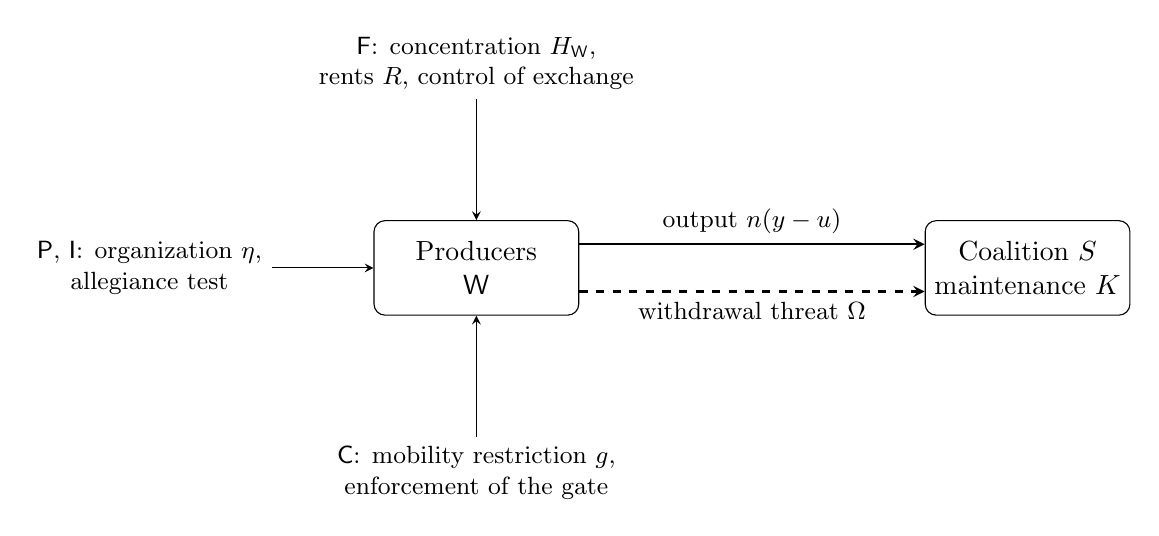
\begin{tikzpicture}[x=1cm,y=1cm,>=stealth]
  \node[draw,rounded corners,minimum width=2.6cm,minimum height=1.2cm,align=center] (W) at (0,0) {Producers\\ $\pW$};
  \node[draw,rounded corners,minimum width=2.6cm,minimum height=1.2cm,align=center] (S) at (7,0) {Coalition $S$\\ maintenance $K$};
  \node[align=center,font=\small] (F) at (0,2.6) {$\pF$: concentration $\HW$,\\ rents $R$, control of exchange};
  \node[align=center,font=\small] (C) at (0,-2.6) {$\pC$: mobility restriction $g$,\\ enforcement of the gate};
  \node[align=center,font=\small,anchor=east] (PI) at (-2.6,0) {$\pP$, $\pI$: organization $\eta$,\\ allegiance test};
  \draw[->,thick] ([yshift=3mm]W.east) -- node[above,font=\small]{output $n(y-u)$} ([yshift=3mm]S.west);
  \draw[->,thick,dashed] ([yshift=-3mm]W.east) -- node[below,font=\small]{withdrawal threat $\Omega$} ([yshift=-3mm]S.west);
  \draw[->] (F) -- (W);
  \draw[->] (C) -- (W);
  \draw[->] (PI) -- (W);
\end{tikzpicture}
\caption{Instruments of the production game. Producers supply output to the coalition and hold a withdrawal threat whose value depends on the coalition's maintenance shortfall; every instrument that lowers producers' terms is held in another pillar.}
\label{fig:instruments}
\end{figure}

\section{Measurement}
\label{sec:measurement}

The model's parameters correspond to observable quantities, though several can be measured only by proxy. Table~\ref{tab:indicators} lists an indicator for each. The list follows the source's rule that weights and codings be preregistered and that no aggregate index be reported for a real country without a documented coding \citep{largo2026hbs}. Largo also warns that measurement invariance across regimes must be tested before indicators are compared \citep{largo2026hbs}. Union density means something different under a party-controlled federation than under independent unions, and the indicators below are meant to be coded with that difference recorded.

\begin{table}[t]
\centering
\small
\caption{Indicators for the parameters of the production game and the components of productive contestability. Each indicator requires a preregistered coding rule before use.}
\label{tab:indicators}
\begin{tabularx}{\textwidth}{@{}L{3.6cm}Y@{}}
\toprule
Quantity & Indicator \\
\midrule
Concentration $\HW$ & Herfindahl index of employment or vacancy shares in local labor markets, the state's share of employment, and the share of farm output sold to a single purchaser \\
Outside option $o$ & Rates of job-to-job transition, wage changes on switching employer, and the legal ability to change employer or residence \\
Mobility restriction $g$ & Statutes and practice on internal passports, residence permits tied to an employer, and debt or land ties \\
Organized weight $\eta$ & Union density, bargaining coverage, legality of strikes, and the independence of unions from the ruling party or employer \\
Rents and maintenance, $R$ and $K$ & Non-tax revenue relative to recurrent spending on administration, courts, security and public information \\
Producer dependence $\xi$ & Share of government revenue raised from domestic taxes and contributions \\
Participation gate $\gamma$ & Rules that condition employment, licenses, credit or market access on political or religious criteria, coded from statute and documented practice \\
Legal access $q^{\mathrm{leg}}$ & Availability, cost and independence of labor and tax adjudication, coded with the components of Part III, Definition 2.4 \\
Income protection $q^{\mathrm{inc}}$ & Replacement rates of unemployment, sickness and old-age insurance \\
Care labor $h$ and carers' fallback $o_h$ & Time-use surveys of unpaid care by sex, coverage of public childcare and paid leave, and women's property and divorce rights \\
\bottomrule
\end{tabularx}
\end{table}

The maintenance requirement $K$ is the hardest quantity to measure. A workable proxy is recurrent spending on the core functions of the other five pillars, excluding transfers and investment, since those are the outlays that cannot be postponed without loss of function. The proxy is imperfect because some transfers are themselves maintenance (pensions to soldiers, stipends to clergy) and because the shortfall cost $\psi$ depends on reserves and borrowing capacity. A preregistered study would fix the proxy and test sensitivity to alternatives.

The model and the comparison yield nine testable hypotheses, listed with their falsifiers in Table~\ref{tab:hypotheses}. Several refine the source's hypotheses H5 and H6 \citep{largo2026hbs}.

\begin{table}[t]
\centering
\small
\caption{Hypotheses for the productive pillar. Each prediction follows from the result named in the second column; the falsifier is the observation that would refute it.}
\label{tab:hypotheses}
\begin{tabularx}{\textwidth}{@{}L{1.0cm}L{2.4cm}YY@{}}
\toprule
 & Basis & Prediction & Falsifier \\
\midrule
HW1 & Source H5, Corollary~\ref{cor:productive-power:gradient} & Higher bargaining coverage weakens the association between employer concentration and lower pay & The concentration gradient is the same at high and low coverage \\
HW2 & Fiscal contract & Governments concede more services and representation where domestic taxes supply more revenue & No relation after conditioning on income, as some tests find \\
HW3 & Proposition~\ref{prop:productive-power:rentier} & The effect of rents on concessions to producers is largest where rents are close to the cost of running the state & The effect is uniform in the ratio of rents to maintenance or largest far from one \\
HW4 & Proposition~\ref{prop:productive-power:domar} & Bondage is more frequent where free exit is valuable and enforcement is cheap & Its incidence is unrelated to both across regions under comparable states \\
HW5 & Everyday resistance & Covert non-compliance rises where open voice is suppressed & Evasion and turnover are unrelated to repression of organization \\
HW6 & Insiders and outsiders & Contestability differs between permanent and precarious workers in encompassing welfare states & No difference in bargaining coverage or income protection between the groups \\
HW7 & Persistence & Compelled labor drafts leave lower consumption in affected districts long after abolition & Comparable drafts show no persistent effect at their boundaries \\
HW8 & Source H6 & Higher tax revenue with accountable provision goes with lower worker vulnerability & Vulnerability rises with provision \\
HW9 & Household application of Proposition~\ref{prop:productive-power:voice} & Unpaid care is shared more evenly where carers' fallback positions are stronger & The division of unpaid care is unrelated to property rights, paid employment and public care \\
\bottomrule
\end{tabularx}
\end{table}

The exit hypotheses, HW1, HW4 and HW7, test how outside options set terms. HW1 is Corollary~\ref{cor:productive-power:gradient}: organization scales the concentration gradient by $1-\eta$, so it should be flatter where bargaining coverage is high. HW4 is the Domar-Brenner condition, and its test requires regional comparisons within one state, so that enforcement institutions are held roughly constant while land-labor ratios and peasant organization vary. HW7 generalizes \citet{dell2010}, whose regression-discontinuity design at the boundary of the draft area is the template.

The fiscal hypotheses, HW2, HW3 and HW8, test the coalition's dependence on producers. HW2 carries the condition that \citet{ross2004} found necessary: the relevant variable is the price of government services, not taxation alone. HW3 is the paper's sharpest new prediction. If most observed variation in rents lies far from the threshold at which rents cover the cost of the state, it reconciles the rentier literature with null findings such as those of \citet{habermenaldo2011}. HW8 is the source's public-goods rival stated for producers: if it holds, high taxation is not evidence of extraction.

The voice hypotheses, HW5, HW6 and HW9, test what happens to producers whose organized weight is low. HW5 follows \citet{scott1985} and the Soviet evidence of \citet{fitzpatrick1994} and \citet{filtzer1986}, and its difficulty is that covert resistance is hard to observe by design. HW6 tests the insider-outsider cleavage that \citet{rueda2005} identified. HW9 follows from the household application of Proposition~\ref{prop:productive-power:voice}, in which a carer's terms rise with the fallback positions emphasized by \citet{agarwal1997}; Lemma~\ref{lem:productive-power:reproduction} explains why that division matters for persistence but does not by itself imply the prediction.

Two identification problems apply to all nine. Organization is endogenous to the terms it is supposed to explain, since producers organize more where they expect gains. Rents, concentration and gates are chosen by coalitions that anticipate producers' responses. Event studies around reforms that change one instrument at a time, of the kind Largo proposes for oversight reforms \citep{largo2026hbs}, are the most direct remedy. Examples include the abolition of tied residence, the legalization of independent unions and the creation of a sovereign fund that removes rents from current budgets.

\section{The Revelation reading}
\label{sec:revelation}

The series reads Revelation 13 and 17 to 18 typologically: the beast is a recurring pattern of power that claims ultimate loyalty, and Babylon is the idolatrous city of every age \citep{bauckham1993,beale1999}. The reading is anchored in the text's first-century setting, the Roman province of Asia, where the imperial cult was a civic institution woven into local life \citep{price1984,friesen2001}. Futurist readings that identify the beast or the mark with a coming government, person, product, technology or payment system are excluded. Their reception history is a record of failed identifications \citep{boyer1992,fuller1995,mcginn1998}. Historicist readings that identified the beast with a particular church or ruler belong to the history of polemic and are excluded for the same reason. The mapping of images to pillars below is a heuristic that aids comparison. It is an interpretive claim of this project, not a settled exegetical result.

The passage most directly relevant to this pillar is Revelation 13:16 and 17 (KJV): ``And he causeth all, both small and great, rich and poor, free and bond, to receive a mark in their right hand, or in their foreheads: And that no man might buy or sell, save he that had the mark, or the name of the beast, or the number of his name.'' The verse does not describe a form of labor. It describes a condition on participation in exchange. Its scope runs across every category of the social order, ``free and bond'' included, so the condition is not the bondage of a class but the gating of everyone's access to buying and selling by a sign of allegiance.

In the terms of Section~\ref{sec:mechanisms}, the verse depicts a closed participation gate, $\gamma=0$, applied to all who withhold allegiance. Proposition~\ref{prop:productive-power:gate} says what such a gate requires and what it yields. It requires control over exchange, a criterion of allegiance and enforcement. In the vision these are distributed across figures: the first beast holds authority and makes war (13:2, 13:4, 13:7); the second beast speaks, performs signs and causes the image of the first to be worshipped (13:12 to 13:15); and the restriction on buying and selling is its economic instrument. The series' heuristic maps these to $\pP$ and $\pC$, to $\pI$, and to the coupling of $\pF$ with $\pW$. The gate also yields a precise result: producers without organization or exit are held to their autarky value. The vision's image of economic exclusion as the sanction for refused allegiance is the limiting case of the model, and it is a limiting case of capture (Proposition B), not of the productive function itself.

The preterist anchor gives the image economic content. \citet{kraybill1996} argued that participation in the maritime trade and trade guilds of Asia Minor entangled Christians in the imperial cult, and that John's vision calls them to withdraw from commerce on those terms. \citet{bauckham1991} read the lament over Babylon in Revelation 18 as an economic critique of Rome. The cargo list of 18:11 to 18:13 runs through luxury goods and ends with ``slaves, and souls of men,'' an indictment of a trade that included human beings. This is literal chattel slavery in the Roman economy. It is the extreme of Table~\ref{tab:bondage} and must not be read as a metaphor for wage labor or taxation. The list also illustrates the relocation lemma: the goods that sustained the imperial center were produced across the provinces and beyond them, and the kings, merchants and shipmasters who lament Babylon's fall (18:9 to 18:19) are those whose wealth depended on that flow.

The text's response to the gate has the shape of Hirschman's triad, though it was written for different purposes. The imperative ``Come out of her, my people'' (18:4) is a call to exit. Faithful witness (11:3 to 11:13) and the ``patience and the faith of the saints'' (13:10) are a form of voice that refuses the demanded loyalty. Loyalty itself is the contested object: the vision depicts a demand for worship, and the faithful are those who give their allegiance elsewhere. \citet{rossing1999} read the contrast between Babylon and the New Jerusalem as a choice between two cities, with an economic critique of imperial Rome at its center. \citet{wink1992} generalized the beast into a domination system present in institutions of every age, a reading congenial to the series' claim that the structure is universal.

The analogy has limits that must be stated. Revelation is apocalyptic literature, and its resolution is divine judgment, not producers' bargaining. \citet{collins1984} argued that the book addresses a crisis that was partly perceived, written to produce catharsis in its readers, and \citet{thompson1990} questioned the extent of persecution under Domitian. The verses supply an image of the limiting case of capture in this pillar, and the model supplies the conditions under which that limit is approached. Neither depends on the other. The analytic claims of this paper stand without the theological reading, and the reading identifies no present institution with the beast.

\section{Objections and scope conditions}
\label{sec:objections}

A Marxian reader will object that production is not one pillar among six but the base on which the others rest, and that the framework flattens class relations into a network. The paper's own results partly concede the point. The latent veto gives production a status that no other pillar has: every other function consumes what this one supplies. But Proposition A asserts only that all six functions exist and depend on one another, not that they carry equal causal weight. Whether production determines the other pillars is a claim about the dependency matrix $B_t$, and it is an empirical question. Largo describes the framework as mid-range institutional theory that treats producers as active rather than as a passive base \citep{largo2026hbs}. The functional-explanation debate in Marxism \citep{cohen1978,elster1985} is a reminder that claims of determination need mechanisms, which is what the production game attempts to supply.

A liberal reader will object that the extraction share mislabels returns to capital and payments for public services, and that market exchange is voluntary. The model accommodates the objection rather than rejecting it. The extraction share is net of services returned. Under competitive conditions, with many employers and free mobility, Lemma~\ref{lem:productive-power:concentration} gives producers the competitive value of their labor, and the liberal benchmark is the case $\HW\to 0$. Capture requires a documented instrument and a documented link to terms. What the model denies is only that voluntariness is a property of exchange as such. It depends on the outside option, and the outside option is shaped by concentration, restriction and gates.

A functionalist objection runs the other way: the paper may have explained the existence of production by its usefulness. It has not. Lemma~\ref{thm:productive-power:necessity} is a condition of persistence. It says that persistent collectives produce, not that their productive institutions exist because they help the collective persist. This is the standard of \citet{hempel1959} and \citet{elster1983}, and the series adopts it throughout. \citet{merton1968} supplies the further point that functional alternatives exist: the same function is met by foraging bands, serf villages, kolkhozes and labor markets.

Unpaid household labor enters the formal results in two places only: the reproduction lemma, which makes care a condition of persistence, and the household application of the bargaining model. The production game itself treats its $n$ producers as identical and sets their terms with the coalition, so it does not derive how care is divided within households or how that division interacts with the terms of paid work. A full treatment would solve the household game jointly with the production game, with each member's fallback set by property, divorce law and access to paid work. This paper states the household game's structure and one hypothesis (HW9) but does not solve it jointly.

The comparative statics are monotone in the parameters, and that monotonicity, not the functional forms, carries the paper's qualitative claims. The functional forms are simple. The production game is stationary, its producers are identical within a group, and the asymmetric Nash solution summarizes rather than models the process of strikes and concessions. Real coalitions face heterogeneous producers, such as citizens and migrants or capital and labor, so the model must be applied group by group.

Two simplifications bear directly on the size of the effects. Reserves and borrowing let coalitions survive withdrawal longer than the stationary shortfall cost suggests, which shrinks the withdrawal premium. The concentration lemma assumes random rematching in proportion to employment shares, which fixes the linear form of the concentration gradient. Relaxations that preserve monotonicity leave the signs of the results intact; their magnitudes require estimation.

The claims about producer power are conditional on human activity remaining necessary for production. Lemma~\ref{lem:productive-power:relocation} keeps the function in place under full automation, but it moves the producer role to the owners and maintainers of equipment, and the latent veto of labor goes with it.

\section{Conclusion}
\label{sec:conclusion}

Production is the one function every other function consumes. From the maintenance axiom, a persistent collective must produce at a positive average rate, and rents, tribute and machines relocate production without removing it. Producers therefore hold a latent veto over any governance system whose outside revenue falls short of its maintenance requirement. The production game prices that veto. Producers' terms rise with their outside option and their organization, fall linearly with the concentration of control over their participation, and lose their withdrawal premium once rents cover the cost of running the state. Restriction of mobility pays exactly when free exit is valuable and enforcement cheap.

Every instrument that lowers producers' terms is exercised in another pillar. The capture of production is therefore always a coupling of production with coercion, allocation, rule-making or legitimation, and never a property of production alone. The comparison of six regime types found the productive function in all of them and its worst forms where control over production was concentrated and coupled to coercion and to control of exchange: under a communist party, a Catholic monarchy and a modern monarchy legitimated by Islam alike. Producers' voice was strongest under social democracy, in some Ottoman guilds and among Burgundian villagers using royal courts. Ideology did not sort the cases. The instruments did.

What remains uncertain is quantitative. None of the model's parameters has been estimated here, and the sharpest prediction, that rents matter most where they nearly cover the cost of the state, awaits a test. The structural claim does not wait on that test. Every governance system in the record depends on those who produce for it, and the image of a world in which no one may buy or sell without the mark describes the condition in which that dependence has been turned entirely against them.

\begin{thebibliography}{131}
\small
\raggedright
\setlength{\itemsep}{2pt}
\bibitem[{Agarwal}(1997)]{agarwal1997}
Agarwal, Bina. 1997. ``Bargaining'' and Gender Relations: Within and Beyond the Household. \emph{Feminist Economics} 3(1): 1-51. doi:10.1080/135457097338799.

\bibitem[{Applebaum}(2003)]{applebaum2003}
Applebaum, Anne. 2003. \emph{Gulag: A History}. Doubleday.

\bibitem[{Azar et~al.}(2022)]{azar2022}
Azar, Jos\'e, Ioana Marinescu, and Marshall Steinbaum. 2022. Labor Market Concentration. \emph{Journal of Human Resources} 57(S): S167-S199. doi:10.3368/jhr.monopsony.1218-9914R1.

\bibitem[{Baer}(1970)]{baer1970}
Baer, Gabriel. 1970. The Administrative, Economic and Social Functions of Turkish Guilds. \emph{International Journal of Middle East Studies} 1(1): 28-50. doi:10.1017/s0020743800023898.

\bibitem[{Barkey}(2008)]{barkey2008}
Barkey, Karen. 2008. \emph{Empire of Difference: The Ottomans in Comparative Perspective}. Cambridge University Press. doi:10.1017/cbo9780511790645.

\bibitem[{Bates and Lien}(1985)]{bates1985}
Bates, Robert H. and Da-Hsiang Donald Lien. 1985. A Note on Taxation, Development, and Representative Government. \emph{Politics \& Society} 14(1): 53-70. doi:10.1177/003232928501400102.

\bibitem[{Bauckham}(1991)]{bauckham1991}
Bauckham, Richard. 1991. The Economic Critique of Rome in Revelation 18. In \emph{Images of Empire}, ed. Loveday Alexander, JSOT Press (JSOTSup 122), pp. 47-90.

\bibitem[{Bauckham}(1993)]{bauckham1993}
Bauckham, Richard. 1993. \emph{The Theology of the Book of Revelation}. Cambridge University Press. doi:10.1017/cbo9780511819858.

\bibitem[{Bayat}(1987)]{bayat1987}
Bayat, Assef. 1987. \emph{Workers and Revolution in Iran: A Third World Experience of Workers' Control}. Zed Books.

\bibitem[{Bayat}(1997)]{bayat1997}
Bayat, Asef. 1997. \emph{Street Politics: Poor People's Movements in Iran}. Columbia University Press.

\bibitem[{Beale}(1999)]{beale1999}
Beale, G. K. 1999. \emph{The Book of Revelation: A Commentary on the Greek Text}. Eerdmans (NIGTC).

\bibitem[{Beblawi and Luciani}(1987)]{beblawiluciani1987}
Beblawi, Hazem and Giacomo Luciani (eds.). 1987. \emph{The Rentier State}. Croom Helm. doi:10.4324/9781315684864.

\bibitem[{Beik}(1985)]{beik1985}
Beik, William. 1985. \emph{Absolutism and Society in Seventeenth-Century France: State Power and Provincial Aristocracy in Languedoc}. Cambridge University Press. doi:10.1017/cbo9780511583797.

\bibitem[{Besley and Persson}(2011)]{besley2011}
Besley, Timothy and Torsten Persson. 2011. \emph{Pillars of Prosperity: The Political Economics of Development Clusters}. Princeton University Press. doi:10.23943/princeton/9780691152684.001.0001.

\bibitem[{Besley and Persson}(2013)]{besley2013}
Besley, Timothy and Torsten Persson. 2013. Taxation and Development. In \emph{Handbook of Public Economics}, vol. 5, Elsevier, pp. 51-110. doi:10.1016/B978-0-444-53759-1.00002-9.

\bibitem[{Boehm}(1999)]{boehm1999}
Boehm, Christopher. 1999. \emph{Hierarchy in the Forest: The Evolution of Egalitarian Behavior}. Harvard University Press. doi:10.2307/j.ctvjf9xr4.

\bibitem[{Boyer}(1992)]{boyer1992}
Boyer, Paul. 1992. \emph{When Time Shall Be No More: Prophecy Belief in Modern American Culture}. Harvard University Press (Belknap). doi:10.2307/jj.41480279.

\bibitem[{Brenner}(1976)]{brenner1976}
Brenner, Robert. 1976. Agrarian Class Structure and Economic Development in Pre-Industrial Europe. \emph{Past \& Present} 70: 30-75. doi:10.1093/past/70.1.30.

\bibitem[{Campbell}(1993)]{campbell1993}
Campbell, John L. 1993. The State and Fiscal Sociology. \emph{Annual Review of Sociology} 19: 163-185. doi:10.1146/annurev.so.19.080193.001115.

\bibitem[{Chaudhry}(1997)]{chaudhry1997}
Chaudhry, Kiren Aziz. 1997. \emph{The Price of Wealth: Economies and Institutions in the Middle East}. Cornell University Press. doi:10.7591/9781501700347.

\bibitem[{Cheng and Selden}(1994)]{cheng1994}
Cheng, Tiejun and Mark Selden. 1994. The Origins and Social Consequences of China's Hukou System. \emph{The China Quarterly} 139: 644-668. doi:10.1017/S0305741000043083.

\bibitem[{Chenoweth and Stephan}(2011)]{chenoweth2011}
Chenoweth, Erica and Maria J. Stephan. 2011. \emph{Why Civil Resistance Works: The Strategic Logic of Nonviolent Conflict}. Columbia University Press.

\bibitem[{Clastres}(1987)]{clastres1987}
Clastres, Pierre. 1987. \emph{Society against the State: Essays in Political Anthropology (1974), trans. Robert Hurley}. Zone Books. doi:10.2307/j.ctv1595m3p.

\bibitem[{Cohen}(1978)]{cohen1978}
Cohen, G. A. 1978. \emph{Karl Marx's Theory of History: A Defence}. Princeton University Press. doi:10.1515/9780691213002.

\bibitem[{Collins}(1984)]{collins1984}
Collins, Adela Yarbro. 1984. \emph{Crisis and Catharsis: The Power of the Apocalypse}. Westminster Press.

\bibitem[{Constable}(1964)]{constable1964}
Constable, Giles. 1964. \emph{Monastic Tithes from Their Origins to the Twelfth Century}. Cambridge University Press.

\bibitem[{Cox et~al.}(2010)]{cox2010}
Cox, Michael, Gwen Arnold, and Sergio Villamayor Tomas. 2010. A Review of Design Principles for Community-based Natural Resource Management. \emph{Ecology and Society} 15(4): 38.

\bibitem[{Craig and Pencavel}(1993)]{craig1993}
Craig, Ben and John Pencavel. 1993. The Objectives of Worker Cooperatives. \emph{Journal of Comparative Economics} 17(2): 288-308. doi:10.1006/jcec.1993.1027.

\bibitem[{Davies and Wheatcroft}(2004)]{davies2004}
Davies, R. W. and Stephen G. Wheatcroft. 2004. \emph{The Years of Hunger: Soviet Agriculture, 1931-1933}. Palgrave Macmillan.

\bibitem[{Dell}(2010)]{dell2010}
Dell, Melissa. 2010. The Persistent Effects of Peru's Mining Mita. \emph{Econometrica} 78(6): 1863-1903. doi:10.3982/ECTA8121.

\bibitem[{Domar}(1970)]{domar1970}
Domar, Evsey D. 1970. The Causes of Slavery or Serfdom: A Hypothesis. \emph{The Journal of Economic History} 30(1): 18-32. doi:10.1017/S0022050700078566.

\bibitem[{Dow}(2003)]{dow2003}
Dow, Gregory K. 2003. \emph{Governing the Firm: Workers' Control in Theory and Practice}. Cambridge University Press. doi:10.1017/CBO9780511615849.

\bibitem[{Drelichman and Voth}(2014)]{drelichman2014}
Drelichman, Mauricio and Hans-Joachim Voth. 2014. \emph{Lending to the Borrower from Hell: Debt, Taxes, and Default in the Age of Philip II}. Princeton University Press.

\bibitem[{Ekelund et~al.}(1996)]{ekelund1996}
Ekelund, Robert B., Robert F. Hebert, Robert D. Tollison, Gary M. Anderson, and Audrey B. Davidson. 1996. \emph{Sacred Trust: The Medieval Church as an Economic Firm}. Oxford University Press.

\bibitem[{Elster}(1983)]{elster1983}
Elster, Jon. 1983. \emph{Explaining Technical Change: A Case Study in the Philosophy of Science}. Cambridge University Press.

\bibitem[{Elster}(1985)]{elster1985}
Elster, Jon. 1985. \emph{Making Sense of Marx}. Cambridge University Press.

\bibitem[{Esping-Andersen}(1985)]{esping1985}
Esping-Andersen, G\"osta. 1985. \emph{Politics against Markets: The Social Democratic Road to Power}. Princeton University Press. doi:10.1515/9781400886203.

\bibitem[{Esping-Andersen}(1990)]{esping1990}
Esping-Andersen, G\"osta. 1990. \emph{The Three Worlds of Welfare Capitalism}. Princeton University Press.

\bibitem[{Evans-Pritchard}(1940)]{evanspritchard1940}
Evans-Pritchard, E. E. 1940. \emph{The Nuer: A Description of the Modes of Livelihood and Political Institutions of a Nilotic People}. Clarendon Press.

\bibitem[{Farber et~al.}(2021)]{farber2021}
Farber, Henry S., Daniel Herbst, Ilyana Kuziemko, and Suresh Naidu. 2021. Unions and Inequality over the Twentieth Century: New Evidence from Survey Data. \emph{The Quarterly Journal of Economics} 136(3): 1325-1385. doi:10.1093/qje/qjab012.

\bibitem[{Filtzer}(1986)]{filtzer1986}
Filtzer, Donald. 1986. \emph{Soviet Workers and Stalinist Industrialization: The Formation of Modern Soviet Production Relations, 1928-1941}. Pluto Press.

\bibitem[{Fitzpatrick}(1994)]{fitzpatrick1994}
Fitzpatrick, Sheila. 1994. \emph{Stalin's Peasants: Resistance and Survival in the Russian Village after Collectivization}. Oxford University Press. doi:10.1093/oso/9780195069822.001.0001.

\bibitem[{Folbre}(1994)]{folbre1994}
Folbre, Nancy. 1994. \emph{Who Pays for the Kids? Gender and the Structures of Constraint}. Routledge. doi:10.4324/9780203168295.

\bibitem[{Freeman and Medoff}(1984)]{freeman1984}
Freeman, Richard B. and James L. Medoff. 1984. \emph{What Do Unions Do?} Basic Books.

\bibitem[{Friedman and Lee}(2010)]{friedman2010}
Friedman, Eli and Ching Kwan Lee. 2010. Remaking the World of Chinese Labour: A 30-Year Retrospective. \emph{British Journal of Industrial Relations} 48(3): 507-533. doi:10.1111/j.1467-8543.2010.00814.x.

\bibitem[{Friesen}(2001)]{friesen2001}
Friesen, Steven J. 2001. \emph{Imperial Cults and the Apocalypse of John: Reading Revelation in the Ruins}. Oxford University Press. doi:10.1093/0195131533.001.0001.

\bibitem[{Fuller}(1995)]{fuller1995}
Fuller, Robert C. 1995. \emph{Naming the Antichrist: The History of an American Obsession}. Oxford University Press. doi:10.1093/acprof:oso/9780195109795.001.0001.

\bibitem[{Gregory and Lazarev}(2003)]{gregory2003}
Gregory, Paul R. and Valery Lazarev (eds.). 2003. \emph{The Economics of Forced Labor: The Soviet Gulag}. Hoover Institution Press.

\bibitem[{Haber and Menaldo}(2011)]{habermenaldo2011}
Haber, Stephen and Victor Menaldo. 2011. Do Natural Resources Fuel Authoritarianism? A Reappraisal of the Resource Curse. \emph{American Political Science Review} 105(1): 1-26. doi:10.1017/S0003055410000584.

\bibitem[{Hacker and Pierson}(2010)]{hackerpierson2010}
Hacker, Jacob S. and Paul Pierson. 2010. \emph{Winner-Take-All Politics: How Washington Made the Rich Richer and Turned Its Back on the Middle Class}. Simon \& Schuster.

\bibitem[{Hanieh}(2011)]{hanieh2011}
Hanieh, Adam. 2011. \emph{Capitalism and Class in the Gulf Arab States}. Palgrave Macmillan. doi:10.1057/9781137495105.

\bibitem[{Hempel}(1959)]{hempel1959}
Hempel, Carl G. 1959. The Logic of Functional Analysis. In \emph{Symposium on Sociological Theory}, ed. Llewellyn Gross, Harper \& Row, pp. 271-307.

\bibitem[{Hertog}(2010)]{hertog2010}
Hertog, Steffen. 2010. \emph{Princes, Brokers, and Bureaucrats: Oil and the State in Saudi Arabia}. Cornell University Press. doi:10.7591/9780801458774.

\bibitem[{Hirschman}(1970)]{hirschman1970}
Hirschman, Albert O. 1970. \emph{Exit, Voice, and Loyalty: Responses to Decline in Firms, Organizations, and States}. Harvard University Press.

\bibitem[{Hoffman}(1996)]{hoffman1996}
Hoffman, Philip T. 1996. \emph{Growth in a Traditional Society: The French Countryside, 1450-1815}. Princeton University Press. doi:10.1515/9780691187204.

\bibitem[{Huber and Stephens}(2001)]{huber2001}
Huber, Evelyne and John D. Stephens. 2001. \emph{Development and Crisis of the Welfare State: Parties and Policies in Global Markets}. University of Chicago Press. doi:10.7208/chicago/9780226356495.001.0001.

\bibitem[{Ibn Khaldun}(1958)]{khaldun1958}
Ibn Khaldun. 1958. \emph{The Muqaddimah: An Introduction to History (1377), trans. Franz Rosenthal}. Pantheon Books / Princeton University Press.

\bibitem[{Kagan}(1981)]{kagan1981}
Kagan, Richard L. 1981. \emph{Lawsuits and Litigants in Castile, 1500-1700}. University of North Carolina Press.

\bibitem[{Kandiyoti}(1988)]{kandiyoti1988}
Kandiyoti, Deniz. 1988. Bargaining with Patriarchy. \emph{Gender \& Society} 2(3): 274-290. doi:10.1177/089124388002003004.

\bibitem[{Kapiszewski}(2001)]{kapiszewski2001}
Kapiszewski, Andrzej. 2001. \emph{Nationals and Expatriates: Population and Labour Dilemmas of the Gulf Cooperation Council States}. Ithaca Press.

\bibitem[{Karaman and Pamuk}(2010)]{karaman2010}
Karaman, K. K{\i}van\c{c} and \c{S}evket Pamuk. 2010. Ottoman State Finances in European Perspective, 1500-1914. \emph{The Journal of Economic History} 70(3): 593-629. doi:10.1017/s0022050710000550.

\bibitem[{Kelly}(1995)]{kelly1995}
Kelly, Robert L. 1995. \emph{The Foraging Spectrum: Diversity in Hunter-Gatherer Lifeways}. Smithsonian Institution Press. doi:10.2307/j.ctv2sx9gc9.

\bibitem[{Kornai}(1986)]{kornai1986}
Kornai, J\'anos. 1986. The Soft Budget Constraint. \emph{Kyklos} 39(1): 3-30. doi:10.1111/j.1467-6435.1986.tb01252.x.

\bibitem[{Kornai}(1992)]{kornai1992}
Kornai, J\'anos. 1992. \emph{The Socialist System: The Political Economy of Communism}. Princeton University Press. doi:10.2307/j.ctv1ddczdr.

\bibitem[{Korpi}(1983)]{korpi1983}
Korpi, Walter. 1983. \emph{The Democratic Class Struggle}. Routledge \& Kegan Paul.

\bibitem[{Korpi and Palme}(1998)]{korpi1998}
Korpi, Walter and Joakim Palme. 1998. The Paradox of Redistribution and Strategies of Equality: Welfare State Institutions, Inequality, and Poverty in the Western Countries. \emph{American Sociological Review} 63(5): 661-687. doi:10.2307/2657333.

\bibitem[{Kraybill}(1996)]{kraybill1996}
Kraybill, J. Nelson. 1996. \emph{Imperial Cult and Commerce in John's Apocalypse}. Sheffield Academic Press (JSNT Supplement 132).

\bibitem[{Kuran}(2011)]{kuran2011}
Kuran, Timur. 2011. \emph{The Long Divergence: How Islamic Law Held Back the Middle East}. Princeton University Press. doi:10.1515/9781400836017.

\bibitem[{Kwass}(2000)]{kwass2000}
Kwass, Michael. 2000. \emph{Privilege and the Politics of Taxation in Eighteenth-Century France}. Cambridge University Press.

\bibitem[{Lapidus}(1978)]{lapidus1978}
Lapidus, Gail Warshofsky. 1978. \emph{Women in Soviet Society: Equality, Development, and Social Change}. University of California Press.

\bibitem[{Largo}(2026)]{largo2026hbs}
Largo, Mateo. 2026. \emph{The Hierarchy of the Beast System: Institutional Power, Elite Coordination, and Economic Dependency Across Political Regimes}. Working paper, 14 October 2026.

\bibitem[{Laslett and Brenner}(1989)]{laslett1989}
Laslett, Barbara and Johanna Brenner. 1989. Gender and Social Reproduction: Historical Perspectives. \emph{Annual Review of Sociology} 15: 381-404. doi:10.1146/annurev.so.15.080189.002121.

\bibitem[{Lee}(1979)]{lee1979}
Lee, Richard B. 1979. \emph{The !Kung San: Men, Women, and Work in a Foraging Society}. Cambridge University Press.

\bibitem[{Lee}(2007)]{lee2007}
Lee, Ching Kwan. 2007. \emph{Against the Law: Labor Protests in China's Rustbelt and Sunbelt}. University of California Press. doi:10.1525/9780520940642.

\bibitem[{Lee}(2013)]{lee2013}
Lee, Richard B. 2013. \emph{The Dobe Ju/'hoansi (4th edition)}. Wadsworth/Cengage Learning.

\bibitem[{Levi}(1988)]{levi1988}
Levi, Margaret. 1988. \emph{Of Rule and Revenue}. University of California Press. doi:10.1525/9780520909540.

\bibitem[{Lindblom}(1977)]{lindblom1977}
Lindblom, Charles E. 1977. \emph{Politics and Markets: The World's Political-Economic Systems}. Basic Books.

\bibitem[{Lipset et~al.}(1956)]{lipset1956}
Lipset, Seymour Martin, Martin A. Trow, and James S. Coleman. 1956. \emph{Union Democracy: The Internal Politics of the International Typographical Union}. Free Press.

\bibitem[{Long}(2026a)]{long2026coercive}
Long, Matthew. 2026a. \emph{Coercive Power and Enforcement}. Part V of The Six Pillars of the Beast System. Working paper, October 2026.

\bibitem[{Long}(2026b)]{long2026financial}
Long, Matthew. 2026b. \emph{Financial Power and Resource Command}. Part I of The Six Pillars of the Beast System. Working paper, October 2026.

\bibitem[{Long}(2026c)]{long2026formalized}
Long, Matthew. 2026c. \emph{The Formalized State: The Hierarchy of the Beast System}. Part VII of The Six Pillars of the Beast System. Working paper, October 2026.

\bibitem[{Long}(2026d)]{long2026ideological}
Long, Matthew. 2026d. \emph{Ideological Power and Legitimation}. Part IV of The Six Pillars of the Beast System. Working paper, October 2026.

\bibitem[{Long}(2026e)]{long2026judicial}
Long, Matthew. 2026e. \emph{Judicial Power and Legal Interpretation}. Part III of The Six Pillars of the Beast System. Working paper, October 2026.

\bibitem[{Long}(2026f)]{long2026political}
Long, Matthew. 2026f. \emph{Political Power and Rule Making}. Part II of The Six Pillars of the Beast System. Working paper, October 2026.

\bibitem[{Mahdavy}(1970)]{mahdavy1970}
Mahdavy, Hossein. 1970. The Patterns and Problems of Economic Development in Rentier States: The Case of Iran. In \emph{Studies in the Economic History of the Middle East}, ed. M. A. Cook, Oxford University Press, pp. 428-467.

\bibitem[{Manning}(2003)]{manning2003}
Manning, Alan. 2003. \emph{Monopsony in Motion: Imperfect Competition in Labor Markets}. Princeton University Press. doi:10.1515/9781400850679.

\bibitem[{Marshall}(1976)]{marshall1976}
Marshall, Lorna. 1976. \emph{The !Kung of Nyae Nyae}. Harvard University Press. doi:10.4159/harvard.9780674180574.

\bibitem[{Martin et~al.}(2009)]{martin2009}
Martin, Isaac William, Ajay K. Mehrotra, and Monica Prasad (eds.). 2009. \emph{The New Fiscal Sociology: Taxation in Comparative and Historical Perspective}. Cambridge University Press. doi:10.1017/CBO9780511627071.

\bibitem[{Marx}(1976)]{marx1976}
Marx, Karl. 1976. \emph{Capital: A Critique of Political Economy, Volume 1 (1867), trans. Ben Fowkes}. Penguin.

\bibitem[{McGinn}(1998)]{mcginn1998}
McGinn, Bernard. 1998. \emph{Antichrist: Two Thousand Years of the Human Fascination with Evil}. Columbia University Press.

\bibitem[{Merton}(1968)]{merton1968}
Merton, Robert K. 1968. \emph{Social Theory and Social Structure (enlarged edition)}. Free Press.

\bibitem[{Michels}(1915)]{michels1915}
Michels, Robert. 1915. \emph{Political Parties: A Sociological Study of the Oligarchical Tendencies of Modern Democracy}. Hearst's International Library.

\bibitem[{Moore}(2004)]{moore2004}
Moore, Mick. 2004. Revenues, State Formation, and the Quality of Governance in Developing Countries. \emph{International Political Science Review} 25(3): 297-319. doi:10.1177/0192512104043018.

\bibitem[{Olson}(1965)]{olson1965}
Olson, Mancur. 1965. \emph{The Logic of Collective Action: Public Goods and the Theory of Groups}. Harvard University Press. doi:10.4159/9780674041660.

\bibitem[{Ostrom}(1990)]{ostrom1990}
Ostrom, Elinor. 1990. \emph{Governing the Commons: The Evolution of Institutions for Collective Action}. Cambridge University Press. doi:10.1017/CBO9780511807763.

\bibitem[{Ostrom}(2010)]{ostromdesign2010}
Ostrom, Elinor. 2010. Beyond Markets and States: Polycentric Governance of Complex Economic Systems. \emph{American Economic Review} 100(3): 641-672. doi:10.1257/aer.100.3.641.

\bibitem[{Pamuk}(2000)]{pamuk2000}
Pamuk, \c{S}evket. 2000. \emph{A Monetary History of the Ottoman Empire}. Cambridge University Press.

\bibitem[{Piketty et~al.}(2018)]{piketty2018}
Piketty, Thomas, Emmanuel Saez, and Gabriel Zucman. 2018. Distributional National Accounts: Methods and Estimates for the United States. \emph{The Quarterly Journal of Economics} 133(2): 553-609. doi:10.1093/qje/qjx043.

\bibitem[{Polanyi}(1944)]{polanyi1944}
Polanyi, Karl. 1944. \emph{The Great Transformation: The Political and Economic Origins of Our Time}. Farrar \& Rinehart.

\bibitem[{Pontusson}(1992)]{pontusson1992}
Pontusson, Jonas. 1992. \emph{The Limits of Social Democracy: Investment Politics in Sweden}. Cornell University Press. doi:10.7591/9781501737541.

\bibitem[{Price}(1984)]{price1984}
Price, S. R. F. 1984. \emph{Rituals and Power: The Roman Imperial Cult in Asia Minor}. Cambridge University Press.

\bibitem[{Prodi}(1987)]{prodi1987}
Prodi, Paolo. 1987. \emph{The Papal Prince: One Body and Two Souls: The Papal Monarchy in Early Modern Europe}. Cambridge University Press.

\bibitem[{Przeworski}(1985)]{przeworski1985}
Przeworski, Adam. 1985. \emph{Capitalism and Social Democracy}. Cambridge University Press. doi:10.1017/cbo9781139171830.

\bibitem[{Quataert and Z\"urcher}(1995)]{quataert1995}
Quataert, Donald and Erik Jan Z\"urcher (eds.). 1995. \emph{Workers and the Working Class in the Ottoman Empire and the Turkish Republic, 1839-1950}. I. B. Tauris.

\bibitem[{Root}(1987)]{root1987}
Root, Hilton L. 1987. \emph{Peasants and King in Burgundy: Agrarian Foundations of French Absolutism}. University of California Press. doi:10.1525/9780520913349.

\bibitem[{Ross}(2001)]{ross2001}
Ross, Michael L. 2001. Does Oil Hinder Democracy? \emph{World Politics} 53(3): 325-361. doi:10.1353/wp.2001.0011.

\bibitem[{Ross}(2004)]{ross2004}
Ross, Michael L. 2004. Does Taxation Lead to Representation? \emph{British Journal of Political Science} 34(2): 229-249. doi:10.1017/S0007123404000031.

\bibitem[{Rossing}(1999)]{rossing1999}
Rossing, Barbara R. 1999. \emph{The Choice between Two Cities: Whore, Bride, and Empire in the Apocalypse}. Trinity Press International (Harvard Theological Studies 48).

\bibitem[{Rothstein}(1996)]{rothstein1996}
Rothstein, Bo. 1996. \emph{The Social Democratic State: The Swedish Model and the Bureaucratic Problem of Social Reforms}. University of Pittsburgh Press. doi:10.2307/jj.13110785.

\bibitem[{Rubin}(2017)]{rubin2017}
Rubin, Jared. 2017. \emph{Rulers, Religion, and Riches: Why the West Got Rich and the Middle East Did Not}. Cambridge University Press. doi:10.1017/9781139568272.

\bibitem[{Rueda}(2005)]{rueda2005}
Rueda, David. 2005. Insider-Outsider Politics in Industrialized Democracies: The Challenge to Social Democratic Parties. \emph{American Political Science Review} 99(1): 61-74. doi:10.1017/S000305540505149X.

\bibitem[{Rueschemeyer et~al.}(1992)]{rueschemeyer1992}
Rueschemeyer, Dietrich, Evelyne Huber Stephens, and John D. Stephens. 1992. \emph{Capitalist Development and Democracy}. University of Chicago Press.

\bibitem[{Sahlins}(1972)]{sahlins1972}
Sahlins, Marshall. 1972. \emph{Stone Age Economics}. Aldine-Atherton. doi:10.4324/9780203037416.

\bibitem[{Scheve and Stasavage}(2016)]{scheve2016}
Scheve, Kenneth and David Stasavage. 2016. \emph{Taxing the Rich: A History of Fiscal Fairness in the United States and Europe}. Princeton University Press. doi:10.1515/9781400880379.

\bibitem[{Scott}(1976)]{scott1976}
Scott, James C. 1976. \emph{The Moral Economy of the Peasant: Rebellion and Subsistence in Southeast Asia}. Yale University Press. doi:10.12987/9780300185553.

\bibitem[{Scott}(1985)]{scott1985}
Scott, James C. 1985. \emph{Weapons of the Weak: Everyday Forms of Peasant Resistance}. Yale University Press. doi:10.12987/9780300153620.

\bibitem[{Scott}(2009)]{scott2009}
Scott, James C. 2009. \emph{The Art of Not Being Governed: An Anarchist History of Upland Southeast Asia}. Yale University Press. doi:10.12987/9780300156522.

\bibitem[{Siegelbaum}(1988)]{siegelbaum1988}
Siegelbaum, Lewis H. 1988. \emph{Stakhanovism and the Politics of Productivity in the USSR, 1935-1941}. Cambridge University Press.

\bibitem[{Silver}(2003)]{silver2003}
Silver, Beverly J. 2003. \emph{Forces of Labor: Workers' Movements and Globalization since 1870}. Cambridge University Press. doi:10.1017/CBO9780511615702.

\bibitem[{Singer}(2008)]{singer2008}
Singer, Amy. 2008. \emph{Charity in Islamic Societies}. Cambridge University Press.

\bibitem[{Thompson}(1990)]{thompson1990}
Thompson, Leonard L. 1990. \emph{The Book of Revelation: Apocalypse and Empire}. Oxford University Press. doi:10.1093/oso/9780195055511.001.0001.

\bibitem[{Timmons}(2005)]{timmons2005}
Timmons, Jeffrey F. 2005. The Fiscal Contract: States, Taxes, and Public Services. \emph{World Politics} 57(4): 530-567. doi:10.1353/wp.2006.0015.

\bibitem[{Vassberg}(1984)]{vassberg1984}
Vassberg, David E. 1984. \emph{Land and Society in Golden Age Castile}. Cambridge University Press.

\bibitem[{Viola}(1996)]{viola1996}
Viola, Lynne. 1996. \emph{Peasant Rebels under Stalin: Collectivization and the Culture of Peasant Resistance}. Oxford University Press. doi:10.1093/oso/9780195101973.001.0001.

\bibitem[{Vitalis}(2007)]{vitalis2007}
Vitalis, Robert. 2007. \emph{America's Kingdom: Mythmaking on the Saudi Oil Frontier}. Stanford University Press. doi:10.1515/9781503626119.

\bibitem[{Walder}(1986)]{walder1986}
Walder, Andrew G. 1986. \emph{Communist Neo-Traditionalism: Work and Authority in Chinese Industry}. University of California Press. doi:10.1525/9780520909007.

\bibitem[{Western and Rosenfeld}(2011)]{western2011}
Western, Bruce and Jake Rosenfeld. 2011. Unions, Norms, and the Rise in U.S. Wage Inequality. \emph{American Sociological Review} 76(4): 513-537. doi:10.1177/0003122411414817.

\bibitem[{Wiessner}(2005)]{wiessner2005}
Wiessner, Polly. 2005. Norm Enforcement among the Ju/'hoansi Bushmen: A Case of Strong Reciprocity? \emph{Human Nature} 16(2): 115-145.

\bibitem[{Wink}(1992)]{wink1992}
Wink, Walter. 1992. \emph{Engaging the Powers: Discernment and Resistance in a World of Domination}. Fortress Press. doi:10.2307/j.ctt1tm7j16.

\bibitem[{Woodburn}(1982)]{woodburn1982}
Woodburn, James. 1982. Egalitarian Societies. \emph{Man (N.S.)} 17(3): 431-451. doi:10.2307/2801707.

\bibitem[{Wright}(2000)]{wright2000}
Wright, Erik Olin. 2000. Working-Class Power, Capitalist-Class Interests, and Class Compromise. \emph{American Journal of Sociology} 105(4): 957-1002. doi:10.1086/210397.
\end{thebibliography}

\end{document}
